%++++++++++++++++++++++++++++++++++++++++
% Don't modify this section unless you know what you're doing!
\documentclass[letterpaper,12pt]{article}
\usepackage{tabularx} % extra features for tabular environment
\usepackage{amsmath}  % improve math presentation
\usepackage{graphicx} % takes care of graphic including machinery
\usepackage[margin=1in,letterpaper]{geometry} % decreases margins
\usepackage{cite} % takes care of citations
\usepackage[final]{hyperref} % adds hyper links inside the generated pdf file
\usepackage{subcaption}
\usepackage{listings}
\usepackage{courier}
\usepackage{float}
\lstset{basicstyle=\footnotesize\ttfamily,breaklines=true}
\hypersetup{
	colorlinks=true,       % false: boxed links; true: colored links
	linkcolor=blue,        % color of internal links
	citecolor=blue,        % color of links to bibliography
	filecolor=magenta,     % color of file links
	urlcolor=blue         
}
\parindent 0pt
\parskip 5pt
%++++++++++++++++++++++++++++++++++++++++


\begin{document}

\lstset{language=Matlab}

\title{Simple Neural Networks for Image Classification\\ \vspace{0.5em} \small{FINAL PROJECT - REPORT}}
\author{Giovanni Ballarin \& Stefanie Bertele}
\date{2018}
\maketitle

\begin{abstract}
Following the paper "\textit{Digit Recognition Using Single Layer Neural Network with Principal Component Analysis}" by Vineet Singh, and Sunil Pranit Lal (2015), our project aims at studying neural networks in the context of image classification tasks. We focus on two different approaches: PCA coupled with fully-connected 1D neural networks of different depths; convolutional neural networks (CNNs) with a simple structure. We work with three different datasets of different visual complexity, and we compare the results.
\end{abstract}


\section{Introduction}

The original approach of the paper by Singh \& Pranit Lal is simple: apply Principal Component Analysis (PCA) to the MNIST dataset, then feed the reduced-dimensionality dataset into a 1-hidden-layer, fully-connected neural network to classify the digits. Before discussing our work, it is important to point out their setup, which is different to what we implement for a number of reasons. \\
Some features are:
\begin{itemize}
\item The dataset used consists of a 60,000 images training set and 10,000 images test set;
\item Using PCA, they document that 281 features retained over 99\% of variance, 103 features retained 95\% of the variance and 53 features retained 90\% of the variance;
\item Their training entail from 500 to 1000 epochs, with a hidden layer size ranging from 31 to 100 nodes, and accuracy rates of $\sim\,96\%-98\%$;
\end{itemize}

\subsection*{Motivation}
Image classification tasks are the first class of visual recognition problems that one has to tackle in computer vision. While the set up in many cases is remarkably easy, and datasets are - at the human eye - quite trivial, lots of effort has been put into devising effective classification algorithms. Even a basic digit classification dataset like MNIST can be complex to solve if it is not approached with the "correct" tools: in particular, while many techniques of machine learning can be used to achieve a relatively high performance, getting to $\sim\,99\%$ accuracy rates is impossible with naive approaches. It is thus important to study what constitutes the \textit{minimal} set of techniques necessary to solve such computer vision task: we focus on neural networks since they have now become the "swiss-army knife" for these kind of problems, and we explore simple architectures.\\

We implement all of our code in MATLAB, and it is openly available \href{https://github.com/giob1994/topics_adv_econometrics/tree/master/Project}{online on Github}.

\subsection*{Datasets}
We consider the following datasets:
	\vspace{1em}
	\begin{itemize}
		\item MNIST
		%\vspace{1em}
		\item notMNIST
		%\vspace{1em}
		\item Fashion MNIST
	\end{itemize}
	\vspace{1em}
Each dataset consists of 10,000 greyscale images that belong to 10 different classes. Each image has the size of $28\times28$ pixels, 784 pixels in total. Visually, these dataset are of increasing complexity: MNIST presents hand-drawn digits from 0 to 9 that consist of few high-contrast lines/strokes; notMNIST instead consists of letters A to J (the first 10 letters of the English alphabet) printed in a number of different fonts, such that there is no single style; finally, Fashion MNIST is a purely visual dataset, featuring clothes of 10 different classes, like jackets, dresses, running shoes or high-heeled shoes. Figure \ref{fig:dataset_example} shows a sample of images taken from the three datasets we just described.

\begin{figure}[hbt]
\centering
\begin{subfigure}{.3\textwidth}
  \centering
  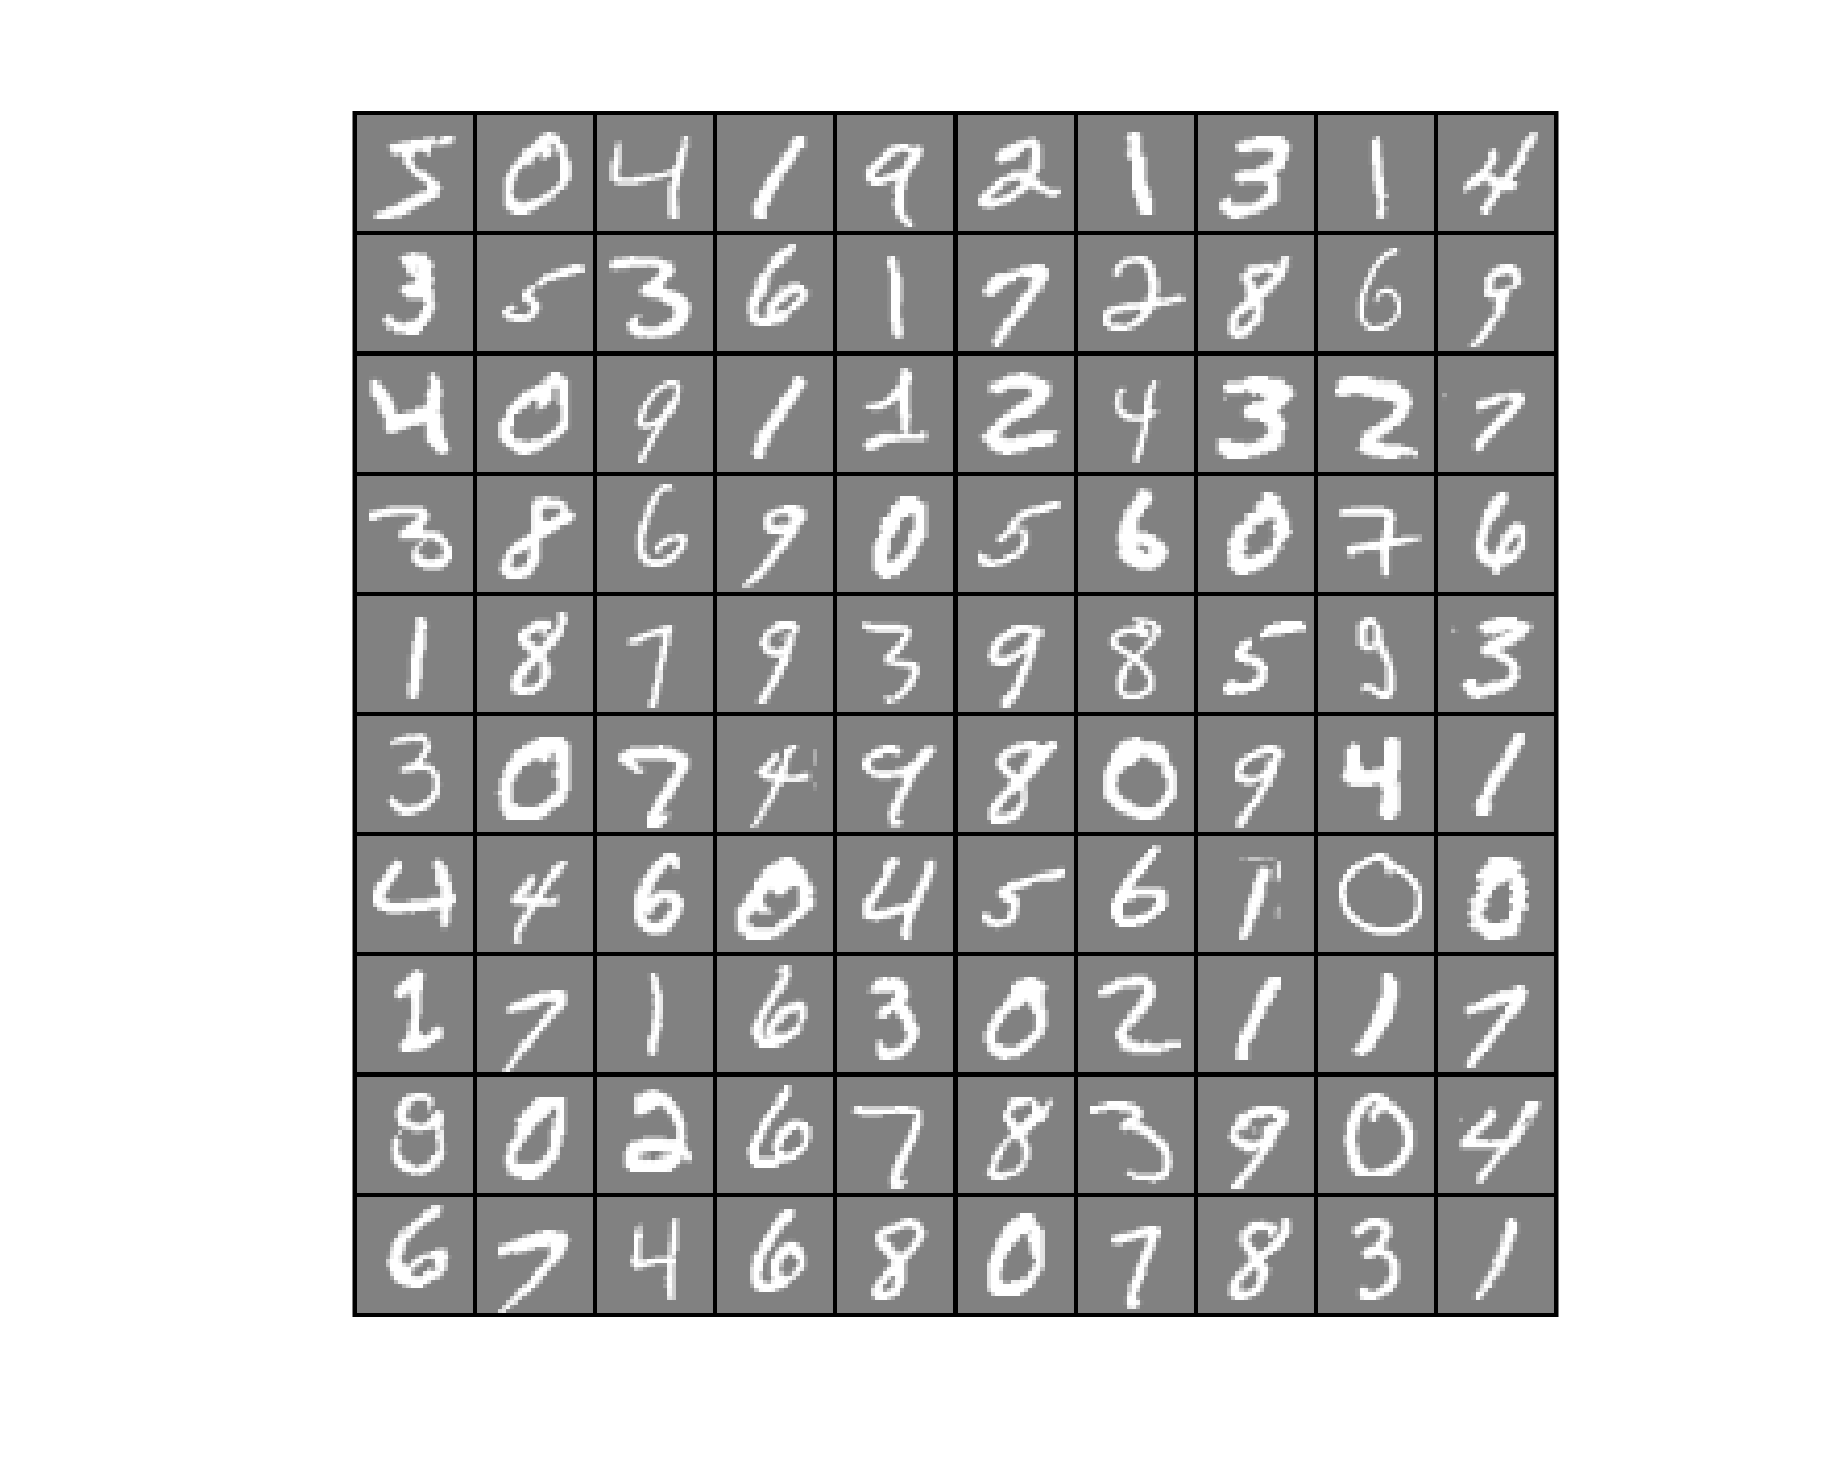
\includegraphics[width=\linewidth]{mnist_example}
  \caption{~}
\end{subfigure}%
\begin{subfigure}{.3\textwidth}
  \centering
  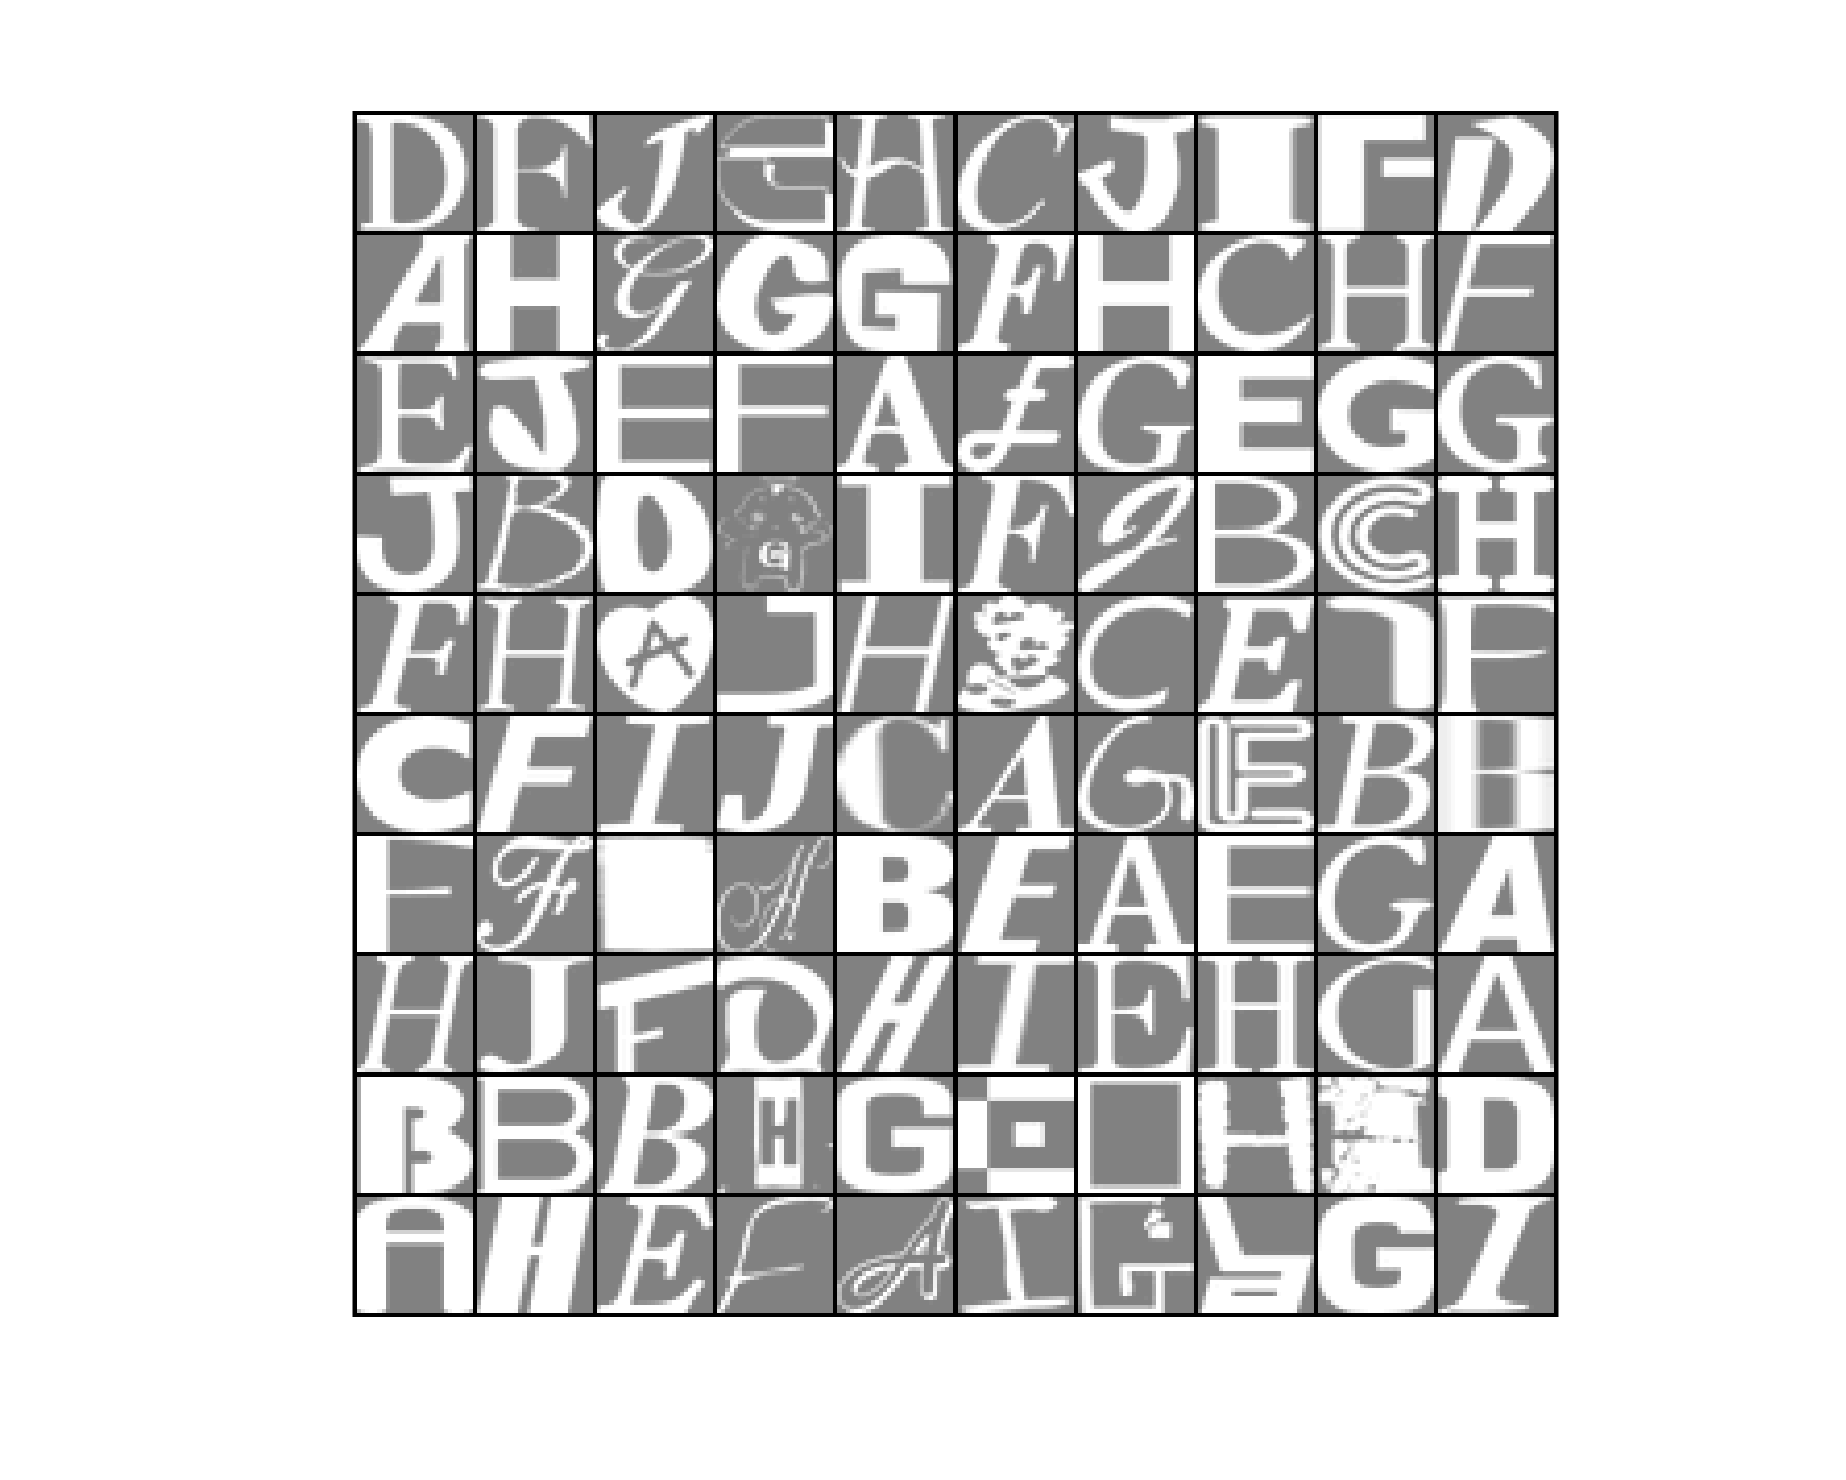
\includegraphics[width=\linewidth]{notMnist_example}
  \caption{~}
\end{subfigure}
\begin{subfigure}{.3\textwidth}
  \centering
  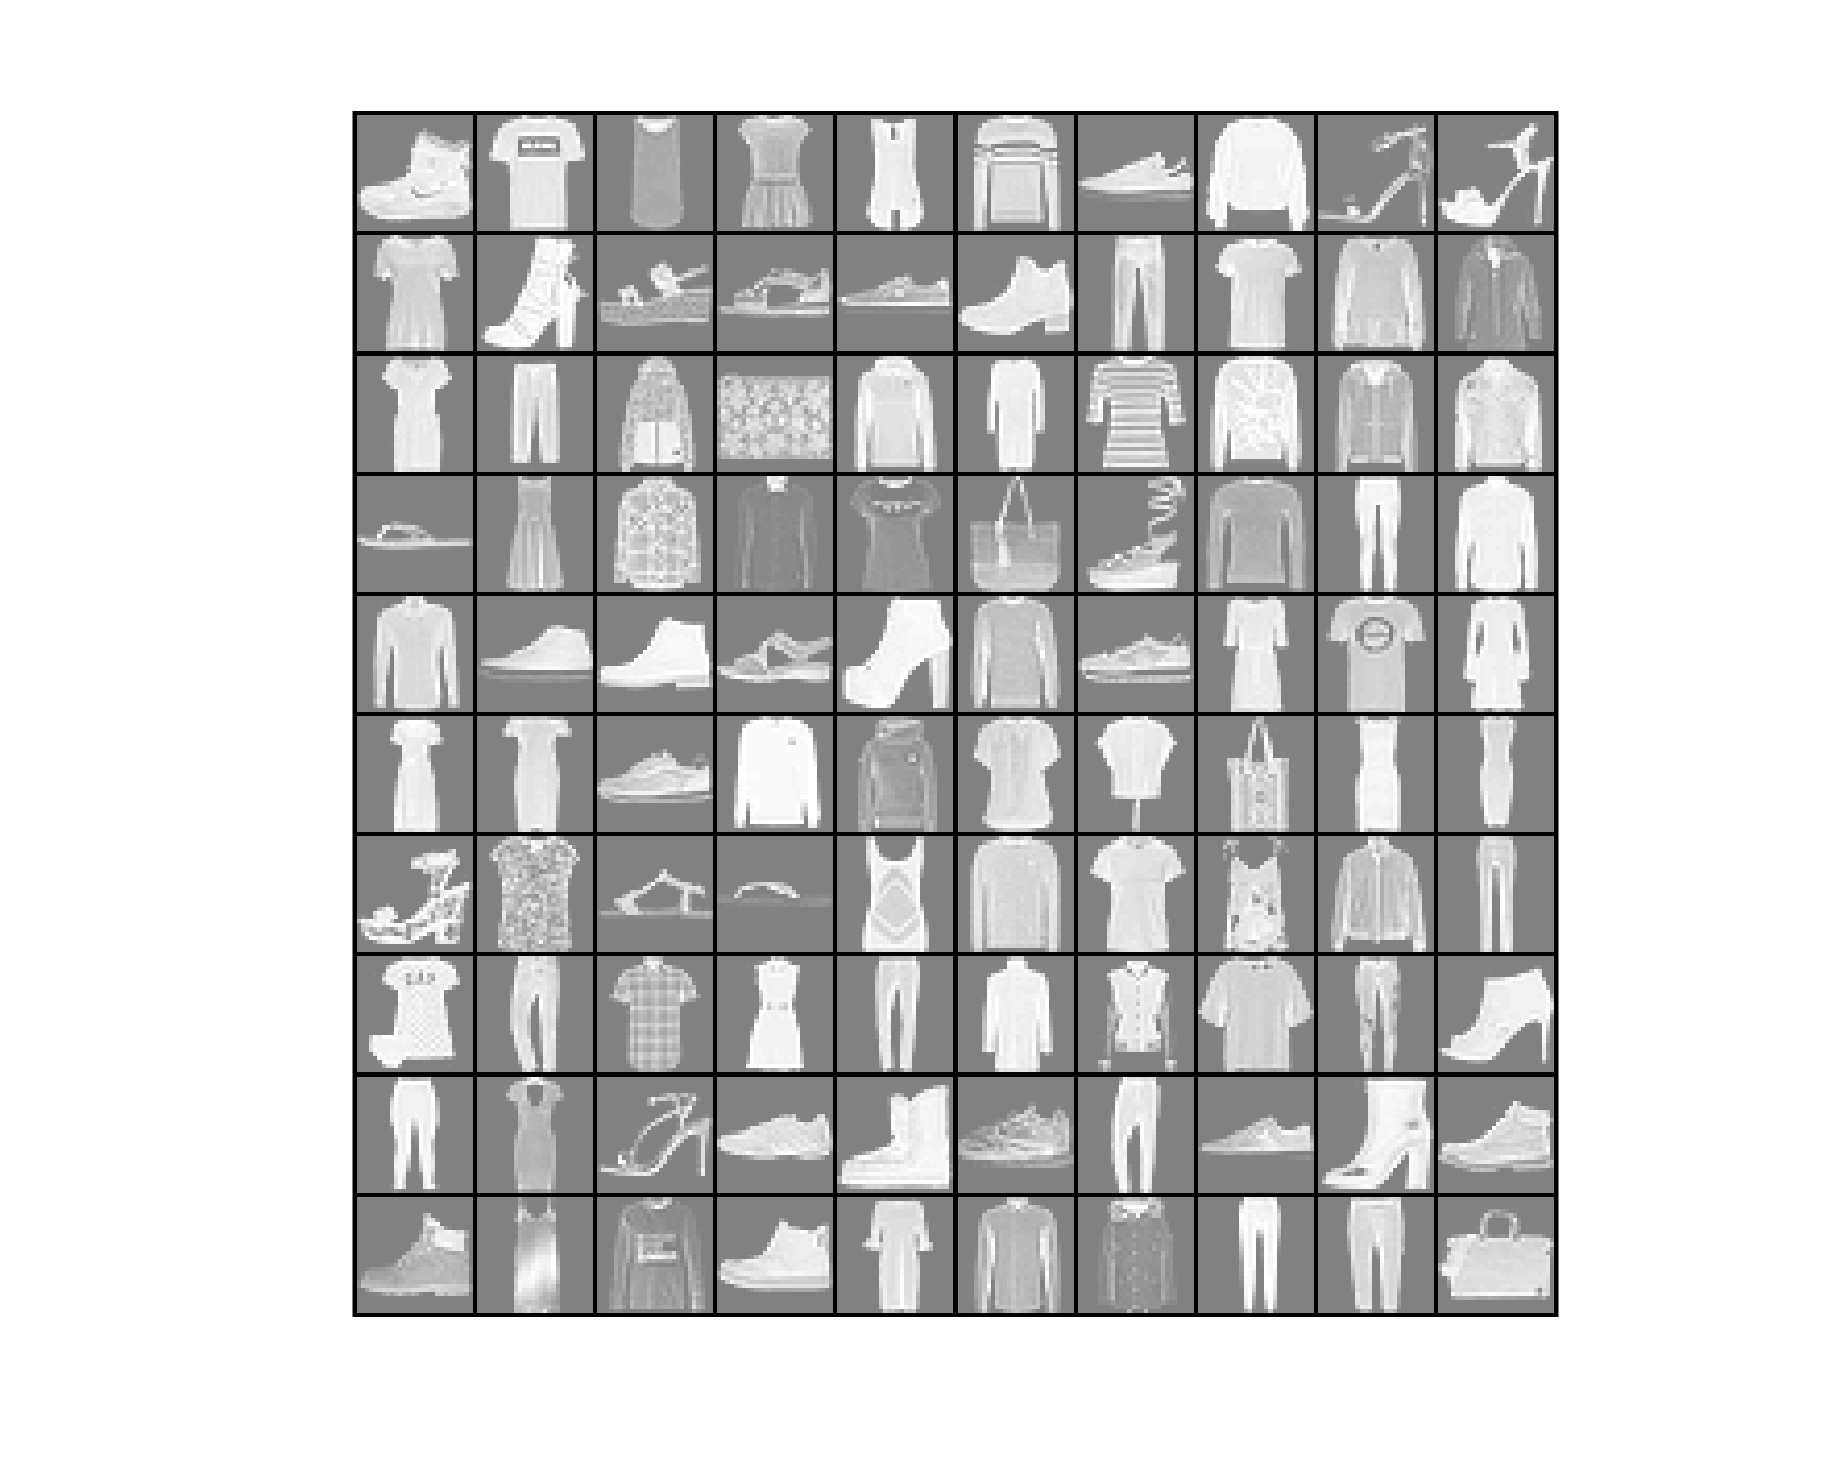
\includegraphics[width=\linewidth]{fashion_example}
  \caption{~}
\end{subfigure}
\caption{Some images taken from the 3 datasets: (a) MNIST; (b) notMNIST; (c) Fashion MNIST.}
\label{fig:dataset_example}
\end{figure}


\section{Techniques}

We decided to expand on the paper in two directions: considering different datasets, but also approaching the more advanced "Convolutional Neural Networks", CNNs, which were developed specifically for vision tasks, and are now found as a building block in practically every neural network architecture that deals with images. 

\subsection*{Fully-Connected Neural Networks in MATLAB}

The Neural Networks Toolbox in MATLAB makes it very simple to define and train simple neural networks. For example, the following code is a valid way of training a fully-connected neural network (FCNN) with 1 hidden layer comprising of 10 neurons: MATLAB will automatically take care of generating matching input/output layers. \\

\begin{lstlisting}
% Load some dataset:
[X_images, y_labels] = dataset;

% Define the neural newtork, and train it on the GPU:
net = feedforwardnet([10], 'trainscg');
net = train(net, X_images, y_labels, 'useGPU', 'yes');

% Let the NN classify the dataset:
predict_labels = net(X_images); 
\end{lstlisting}

\subsection*{Training Algorithms for Fully-Connected Neural Networks}

At the beginning of our project, we were faced with the problem of finding a "good" algorithm to train the fully-connected neural networks we were going to use to classify the Principal Component Analysis outputs. Since our code was implemented in MATLAB, there a number of options available, which we decided to explore beforehands. 

\begin{table}[!ht]
\centering
  \begin{tabular}{|l|c|c|c|}
  	\hline
    Algorithm & Training Error & Test Error & Time(s)\\
    \hline
    \hline
    'trainlm'*  & --- & --- & ---\\
    'trainbr'  & --- & --- & ---\\
    'trainbfg'  & --- & --- & ---\\
    'trainrp'  &    0.70211  &   0.717    &      5.5384\\
    'trainscg'  &  0.070556  &   0.099    &      20.089\\
    'traincgb'  &  0.072111  &   0.102     &     28.357\\
    'traincgf'  &   0.10089   &  0.123    &      33.485\\
    'traincgp' &   0.069667  &   0.099    &      36.416\\
    'trainoss'  &   0.15922  &   0.173     &     48.149\\
    'traingdx'  &   0.32044  &   0.328     &     4.2746\\
    'traingdm'  &   0.89878  &   0.886    &     0.57124\\
    'traingd'   &   0.45789  &   0.442    &      25.565\\
    \hline
  \end{tabular}
  \vspace{0.5em}
  \caption{Performance comparison between the training options for the MATLAB function 'train(...)'. \footnotesize{(* 'trainlm' is the default training algorithm.)} }
  \label{table:train_algorithms}
\end{table}

Table \ref{table:train_algorithms} shows the full list of available algorithms for training the fully-connected neural networks. In MATLAB, one can choose a specific training routine when defining the network: in the previous code, we choose to train using "Scaled Conjugate Gradient" ('trainscg'). \\
As can be seen from Table \ref{table:train_algorithms}, the first three algorithms were excluded directly from testing: this is because "Levemberg-Marquardt" ('trainlm', the default algorithm), "Bayesian Regularization" ('trainbr') and "BFGS Quasi-Newton" ('trainbfg') all performed incredibly poorly on our test machine, time-wise. In fact, for some of the multi-layer architecture we will be using, we could not get these training algorithms to converge in a reasonable amount of time. In the end, we decided to use the Scaled Conjugate Gradient algorithm, as it is the best compromise between accuracy (it routinely produced one of the 3 best training errors, and usually scored the best test error performances) and computation time (while some other methods like Gradient Descend are faster, they had much worse performances).

\subsection*{Principal Component Analysis}
The aim of PCA is to reduce the dimensionality of the data, without loosing the most relevant features. We start with a vector space consisting of 784 dimensions, which is the total amount of pixels per image, that is we vectorise images by stacking all pixels values in one vector. This vector space can be reduced by getting rid of the redundant dimensions, which are the ones accounting for the least variance. The number of dimensions left are then equal to the number of principal components choose for the PCA. In order to do so, we first demeaned the data and computed the covariance matrix: then the eigenvectors of the covariance matrix are sorted in descending order of the corresponding eigenvalues. Finally, the data is projected onto the new "reduced" vector space by multiplying each image vector by the first $K$ eigenvectors.\\
We agreed on four levels of explanatory power of the variance: 50\%, 75\%, 85\% and 95\%. This means that for each level of explanatory power of the variance we compute the number of principal components needed.\\
We analyzed six different structures of fully-connected neural network architectures: a single layer neural network consisting out of 10, 25 or 100 neurons; a two layer neural network including 25 neurons in the first and 15 neurons in the second layer; and two neural networks architectures with three layers with either 25 neurons in the first, 20 neurons in the second and 15 neurons in the third layer or a very complex one with 100 neurons in the first, 50 neurons in the second and 20 neurons in the third layer.\\
First, the necessary number of principal components for each level of explained variance is computed ,and thereafter the different architectures of the neural network are trained and evaluated. This is done for all three datasets. 

\subsubsection*{2D Fourier Transform for Fashion MNIST}
Fashion MNIST is pre-treated with the 2D Fourier Transform (2D FT) to move the data into frequency domain: this process removes the spatial information of the image, but at the same time allows to achieve lower test and training errors than without the use of the 2D FT. A visual example of the result of the 2D FT on Fashion MNIST can be seen in Figure \ref{fig:2dft}. Without 2D Fourier Transform, even the most complex fully-connected neural network architecture can only achieve $\sim 70\%$ training error, which is too high to be comparable with the ones of MNIST and notMNIST datasets.

\begin{figure}[!ht]
\centering
%\textbf{2D Fourier Transform \\}
\vspace{1em}
\begin{subfigure}{.35\textwidth}
  \centering
  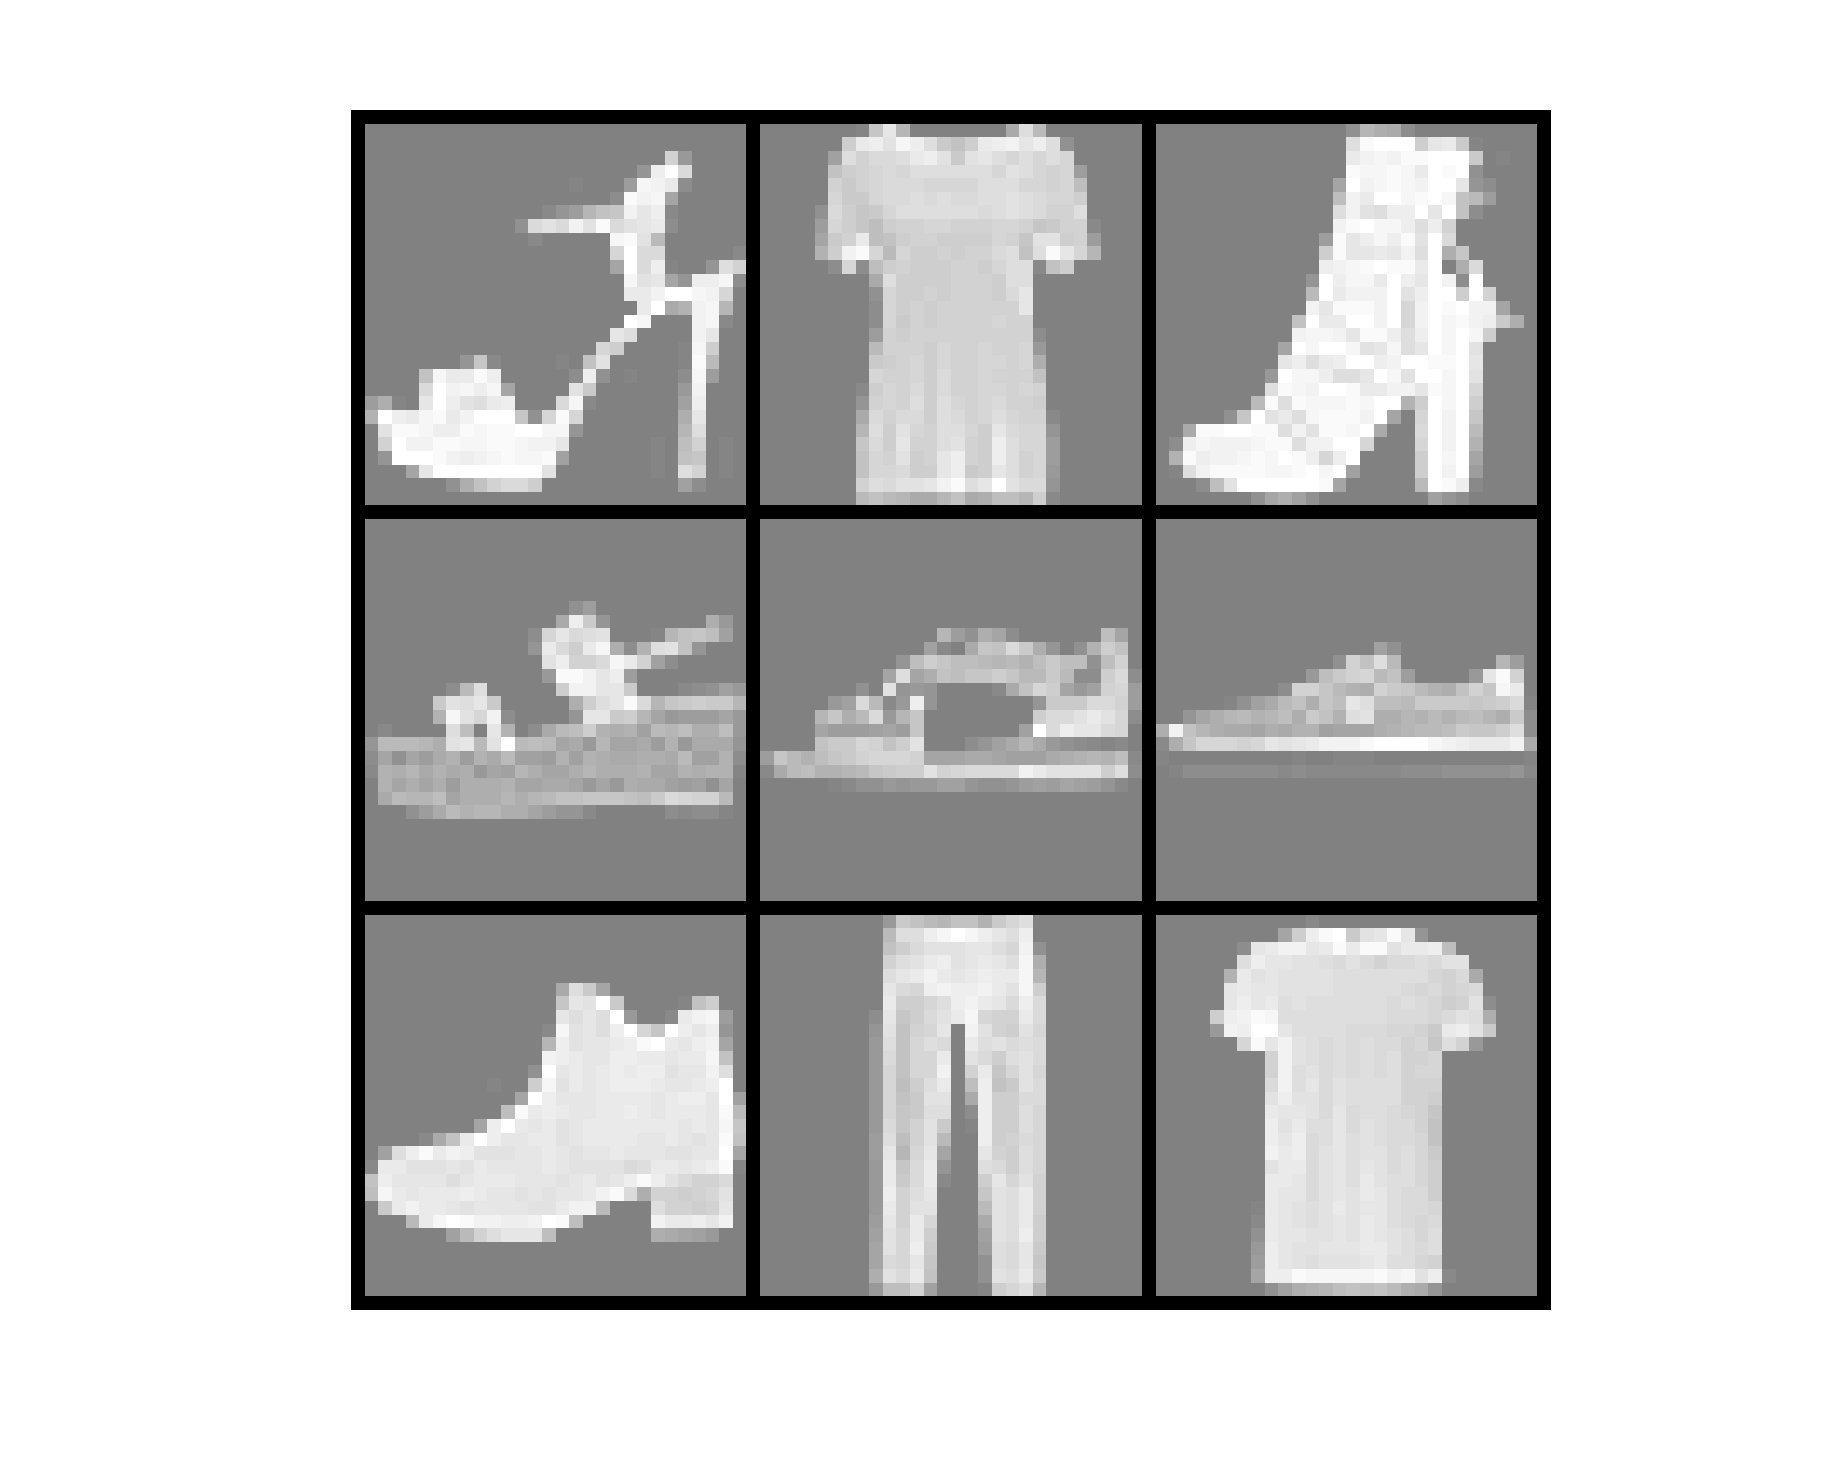
\includegraphics[width=\linewidth]{fashion_raw}
  \caption{~}
\end{subfigure}
\begin{subfigure}{.35\textwidth}
  \centering
  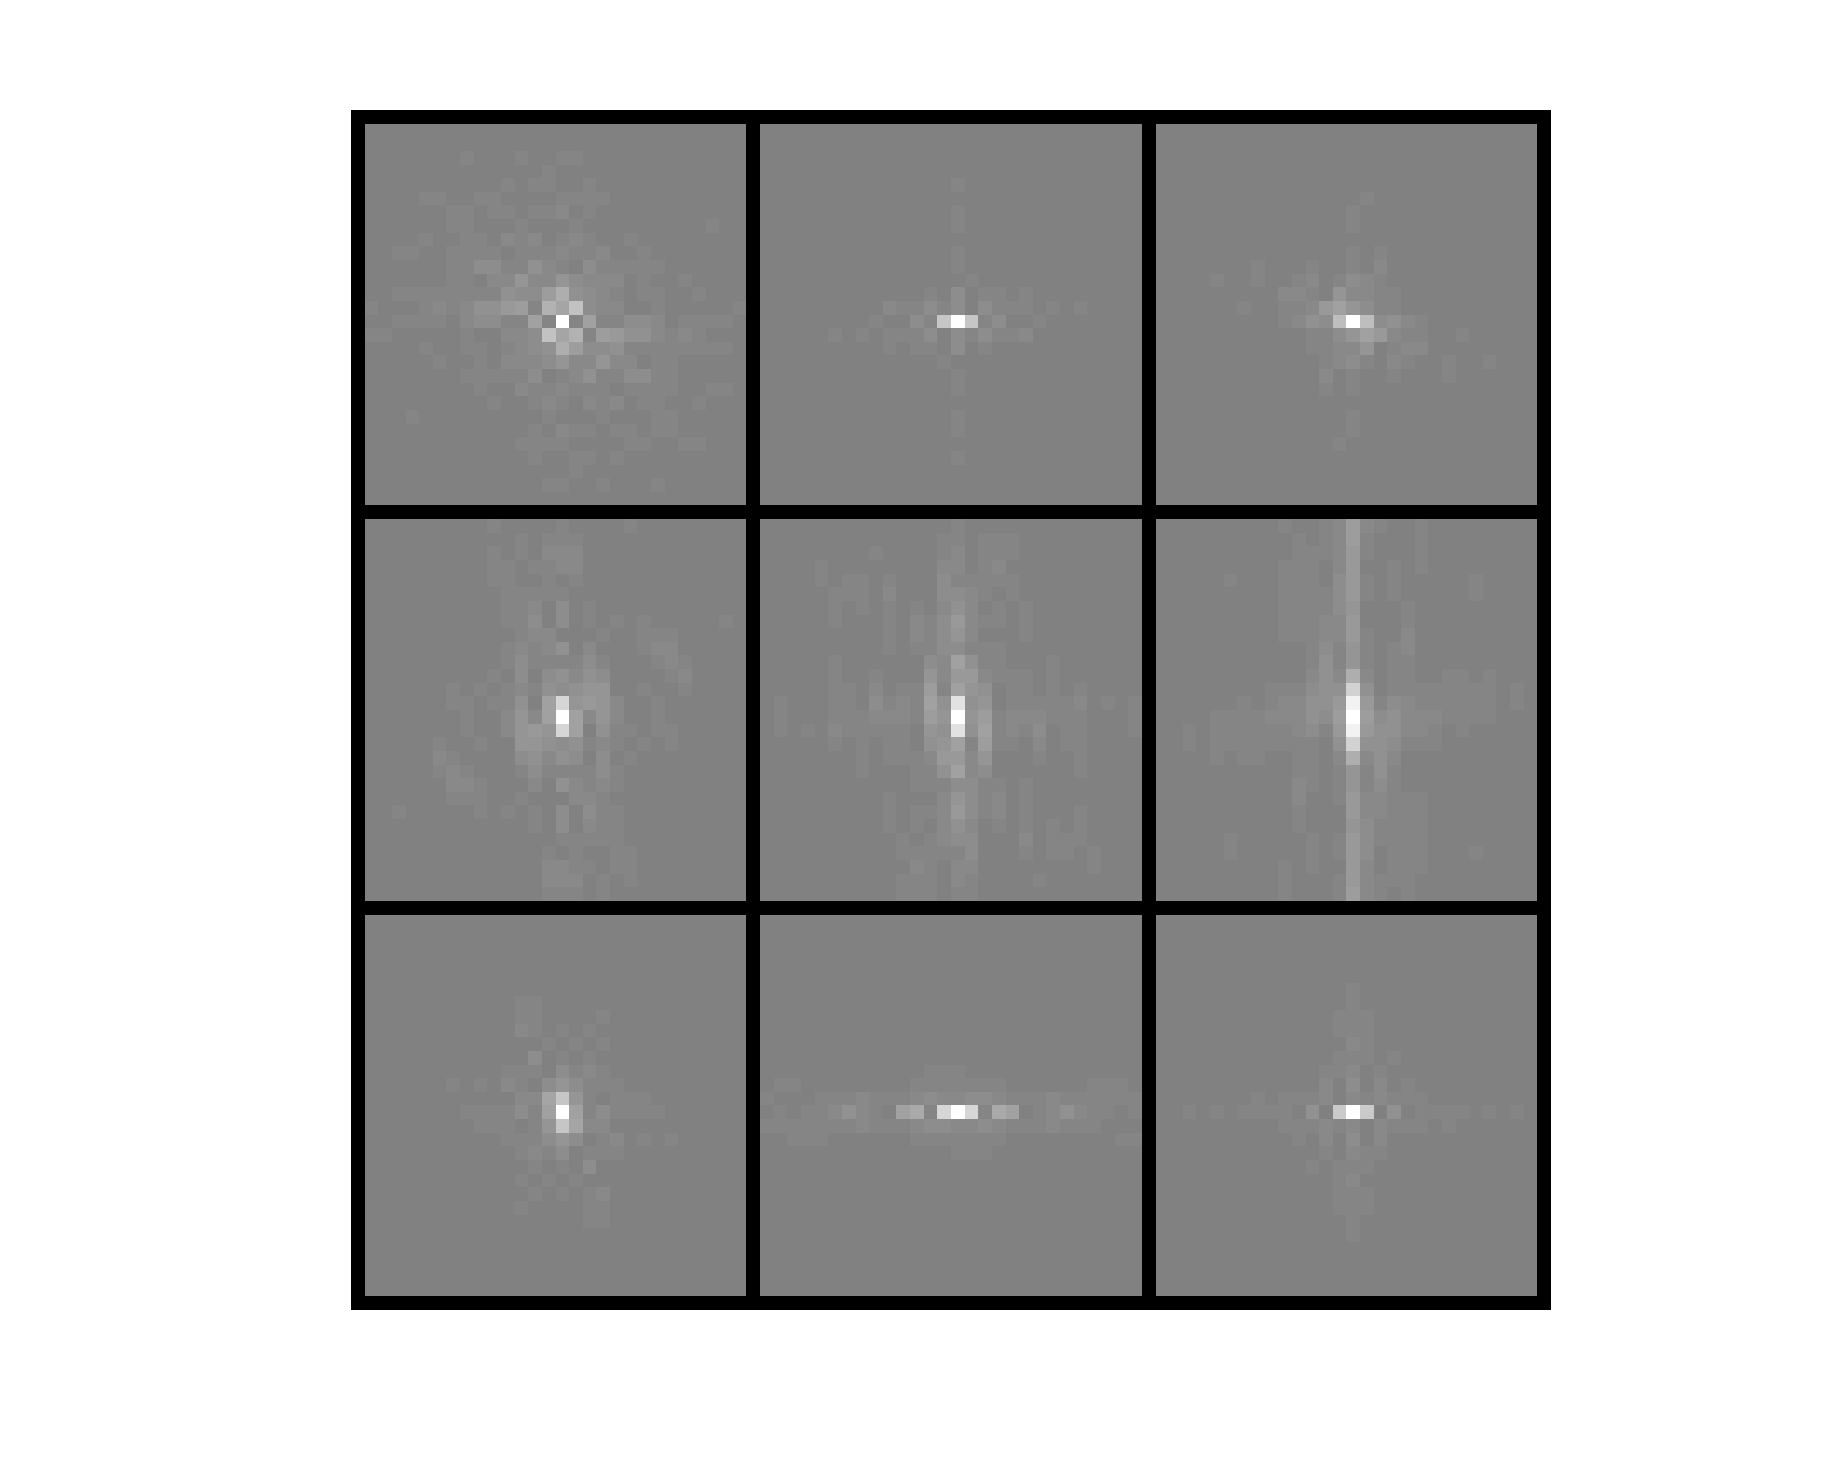
\includegraphics[width=\linewidth]{fashion_ft2}
  \caption{~}
\end{subfigure}
\caption{2D Fourier Transform applied on the Fashion MNIST dataset.}
\label{fig:2dft}
\end{figure}

\subsection*{Convolutional Neural Networks}

Convolutional neural networks, abbreviated "CNNs", are a variation of multilayer perceptrons that was designed to mimic the visual processing of living organisms. Specifically, they try to account for the spatial information that is intrinsic in any image input: the relative position of each pixel to the ones around it is a visually fundamental piece on information that simply fully-connected neural networks fail to exploit, because they have no concept of "local" information. On the other hand, each CNN layer is constructed with a number of filters: each filter is simply a 2D matrix of parameter used to make a convolution with the image, producing an output that is called filter bank. On the application side, CNNs have notable advantages compared to fully-connected NN:
\begin{itemize}
		\item Each filter is usually small in size (e.g. $5\times5$), thus CNNs have considerably less parameters to train to achieve results comparable to those of FCNN;
		\item CNNs preserve the spatial nature of 2D signals like images or video, allowing for more effective feature recognition. 
\end{itemize} 
Clearly, given $j$ filters, the output of a convolutional layer is $j$ filter banks. Also, it is important to notice that given the size of the input, and the size of the filter, the dimension of each output filter bank is determined, and the only "free" parameter is the number of filters.\\
For our project, we consider 4 CNN architectures of increasing complexity. Figure \ref{fig:CNN_archi} shows graphically the structures we chose for the convolutional neural network part of our project. \\

In MATLAB, the Neural Network Toolbox makes it easy to train and test convolutional neural networks: in the following code example, we train a 1 layer CNN on an image dataset.\\

\begin{lstlisting}
% Define the CNN architecture:
CNN_layers = [ ...
                % Input layer:
                imageInputLayer([28, 28, 1]);
                % Convolution layer, 4 [5x5] filters, padding of 2 pixels: 
                convolution2dLayer(5, 4, 'Padding', 2);
                reluLayer;
                % Fully-connected layer for classification:
                fullyConnectedLayer(10);
                softmaxLayer();
                % Output layer:
                classificationLayer();
              ];
              
% Define training options:
options = trainingOptions(
    % Use Stochastic Gradient Descend with Momentum for training:
    'sgdm',...
    'LearnRateSchedule', 'piecewise', ...
    'LearnRateDropFactor', 0.2, ...
    'LearnRateDropPeriod', 5, ...
    % Use maximum of 20 epochs for training:
    'MaxEpochs', 20, ...
    'MiniBatchSize', 64, ...
    'L2Regularization',0.0005, ...
    % Choose the validation data:
    'ValidationData', {valImages, valLabels}, ...
    'ValidationPatience', 10 ...
);

% Train the network:
CNN_net = trainNetwork( trainImages, trainLabels, ...
                        CNN_layers, ...
                        options 
                      );
                
% Use the network for prediction:
CNN_net_predict = classify( CNN_net, imagesToClassify );
\end{lstlisting}

\begin{figure}[p]
\centering
\textbf{CNN Architectures\\}
\vspace{2em}
{Architecture 1\\}
\vspace{0.5em}
  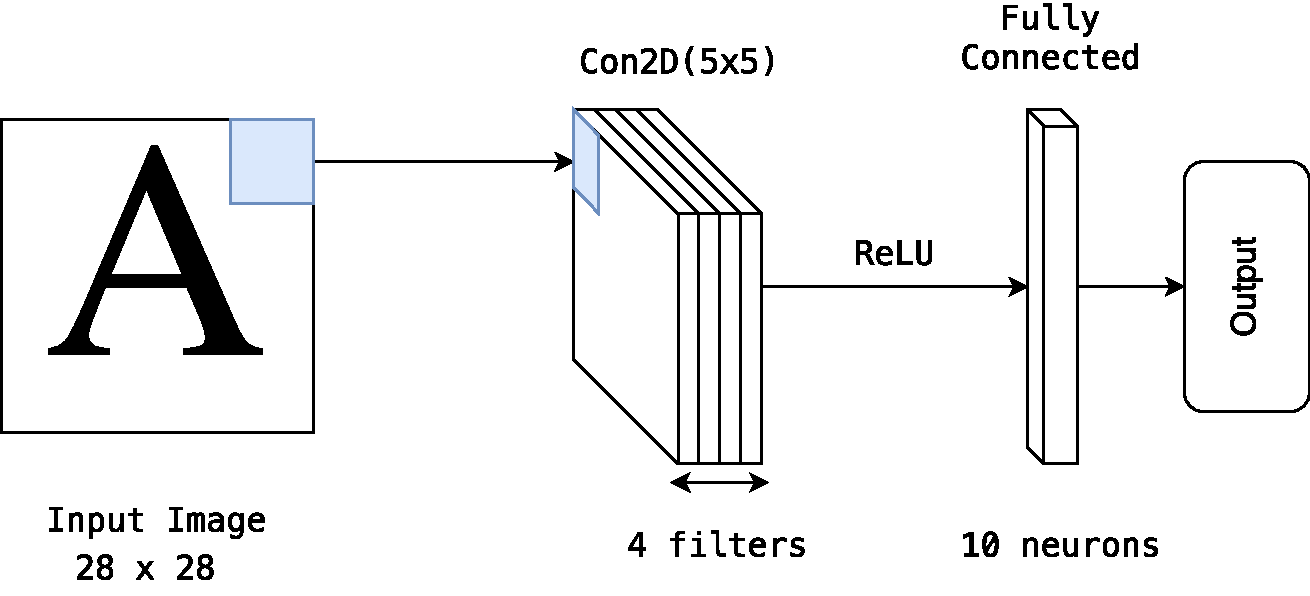
\includegraphics[width=0.5\linewidth]{diag_1}
\vfill
\vspace{1em}
{Architecture 2\\}
\vspace{0.5em}
  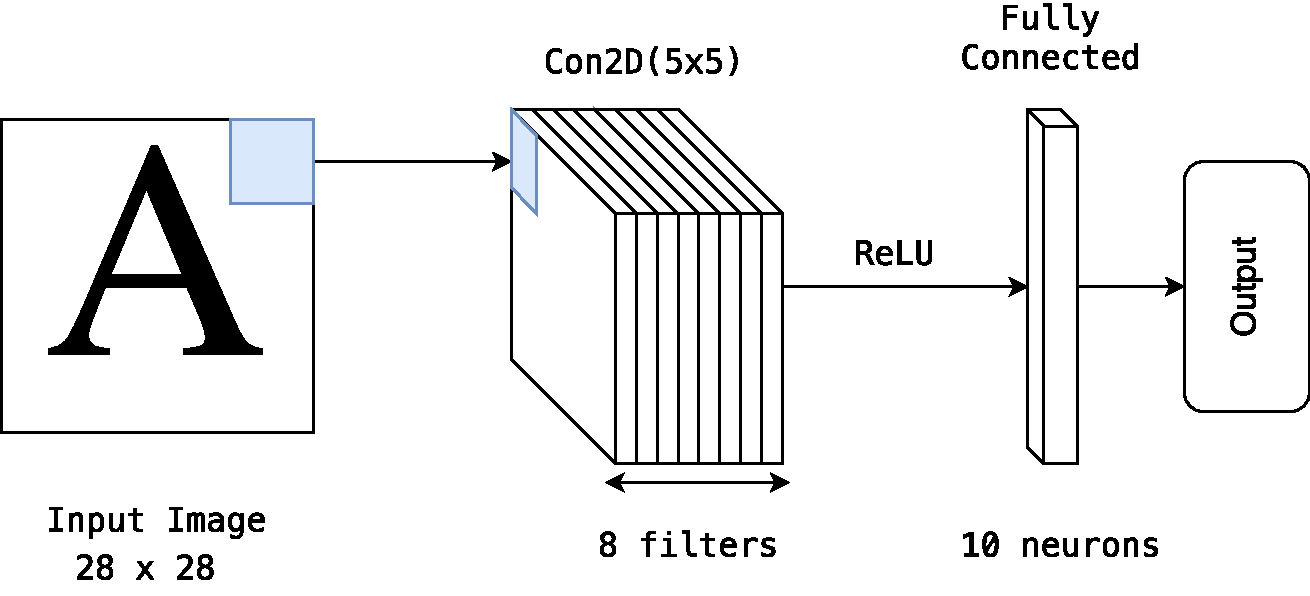
\includegraphics[width=0.5\linewidth]{diag_2}
\vfill
\vspace{1em}
{Architecture 3\\}
\vspace{0.5em}
  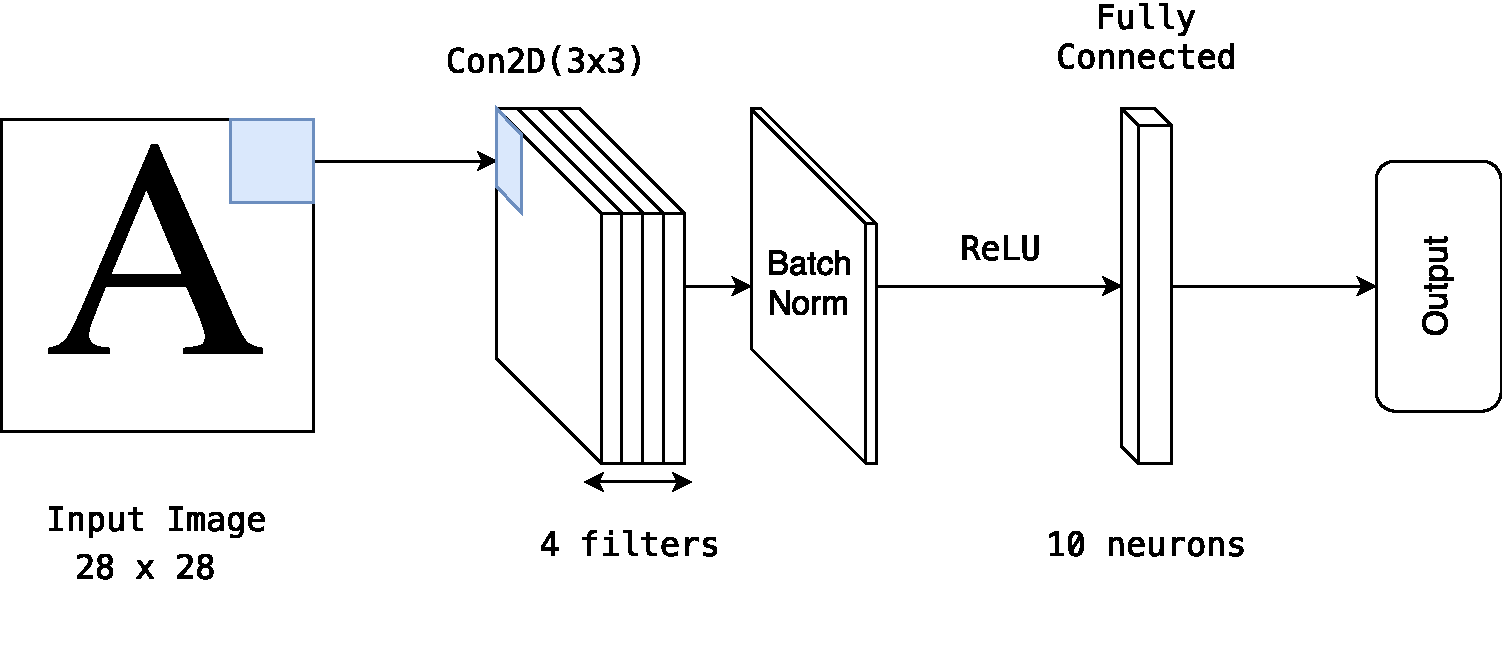
\includegraphics[width=0.55\linewidth]{diag_3}
\vfill
\vspace{1em}
{Architecture 4\\}
\vspace{0.5em}
  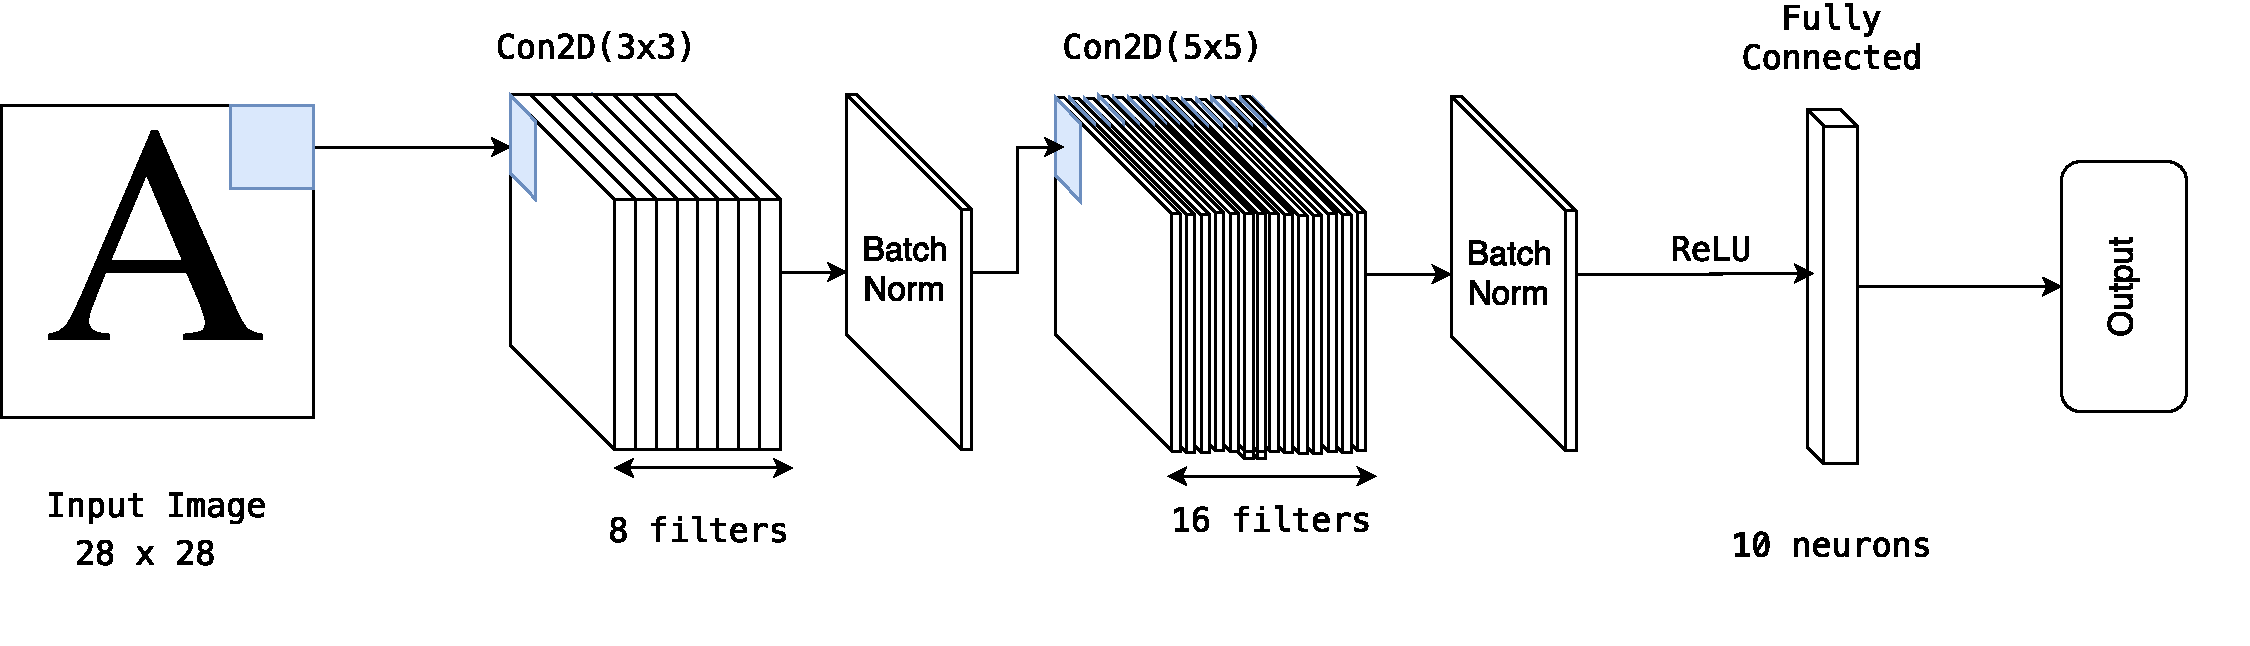
\includegraphics[width=0.9\linewidth]{diag_4}
\vfill
\vspace{2em}
\caption{CNN architectures used in our project, listen in order of complexity/sophistication.}
\label{fig:CNN_archi}
\end{figure}

\section{Results}

\subsection*{PCA}
Although Fashion MNIST appears to be visually the most complex dataset followed by notMNIST and MNIST, the number of principal components needed seems to be decreasing in visual complexity for these datasets. Obviously, the higher the level of variance explained is set, the more principal components are needed for all datasets. For MNIST the lowest training error, but the highest test error are achieved, so we cannot confirm the results obtained by Singh and Lal. The very simple neural networks consisting out of a single layer with just 10 or 25 neurons perform best, whereas more deep neural networks perform worse. This is not the case for notMNIST anymore, where sometimes very simple one layer networks work best, but sometimes the most complex one works best. The training error is higher than for MNIST, but the test error decreases, meaning that the worst test error for notMNIST is even lower than the best test error for MNIST. Fashion MNIST yields an even higher training error with an even higher test error. This relationship of increasing training error and decreasing test error is somehow counterintuitive and puzzling and we cannot explain it.  

\begin{figure}[p]
\centering
\textbf{Results: PCA + FCNN on MNIST dataset}
  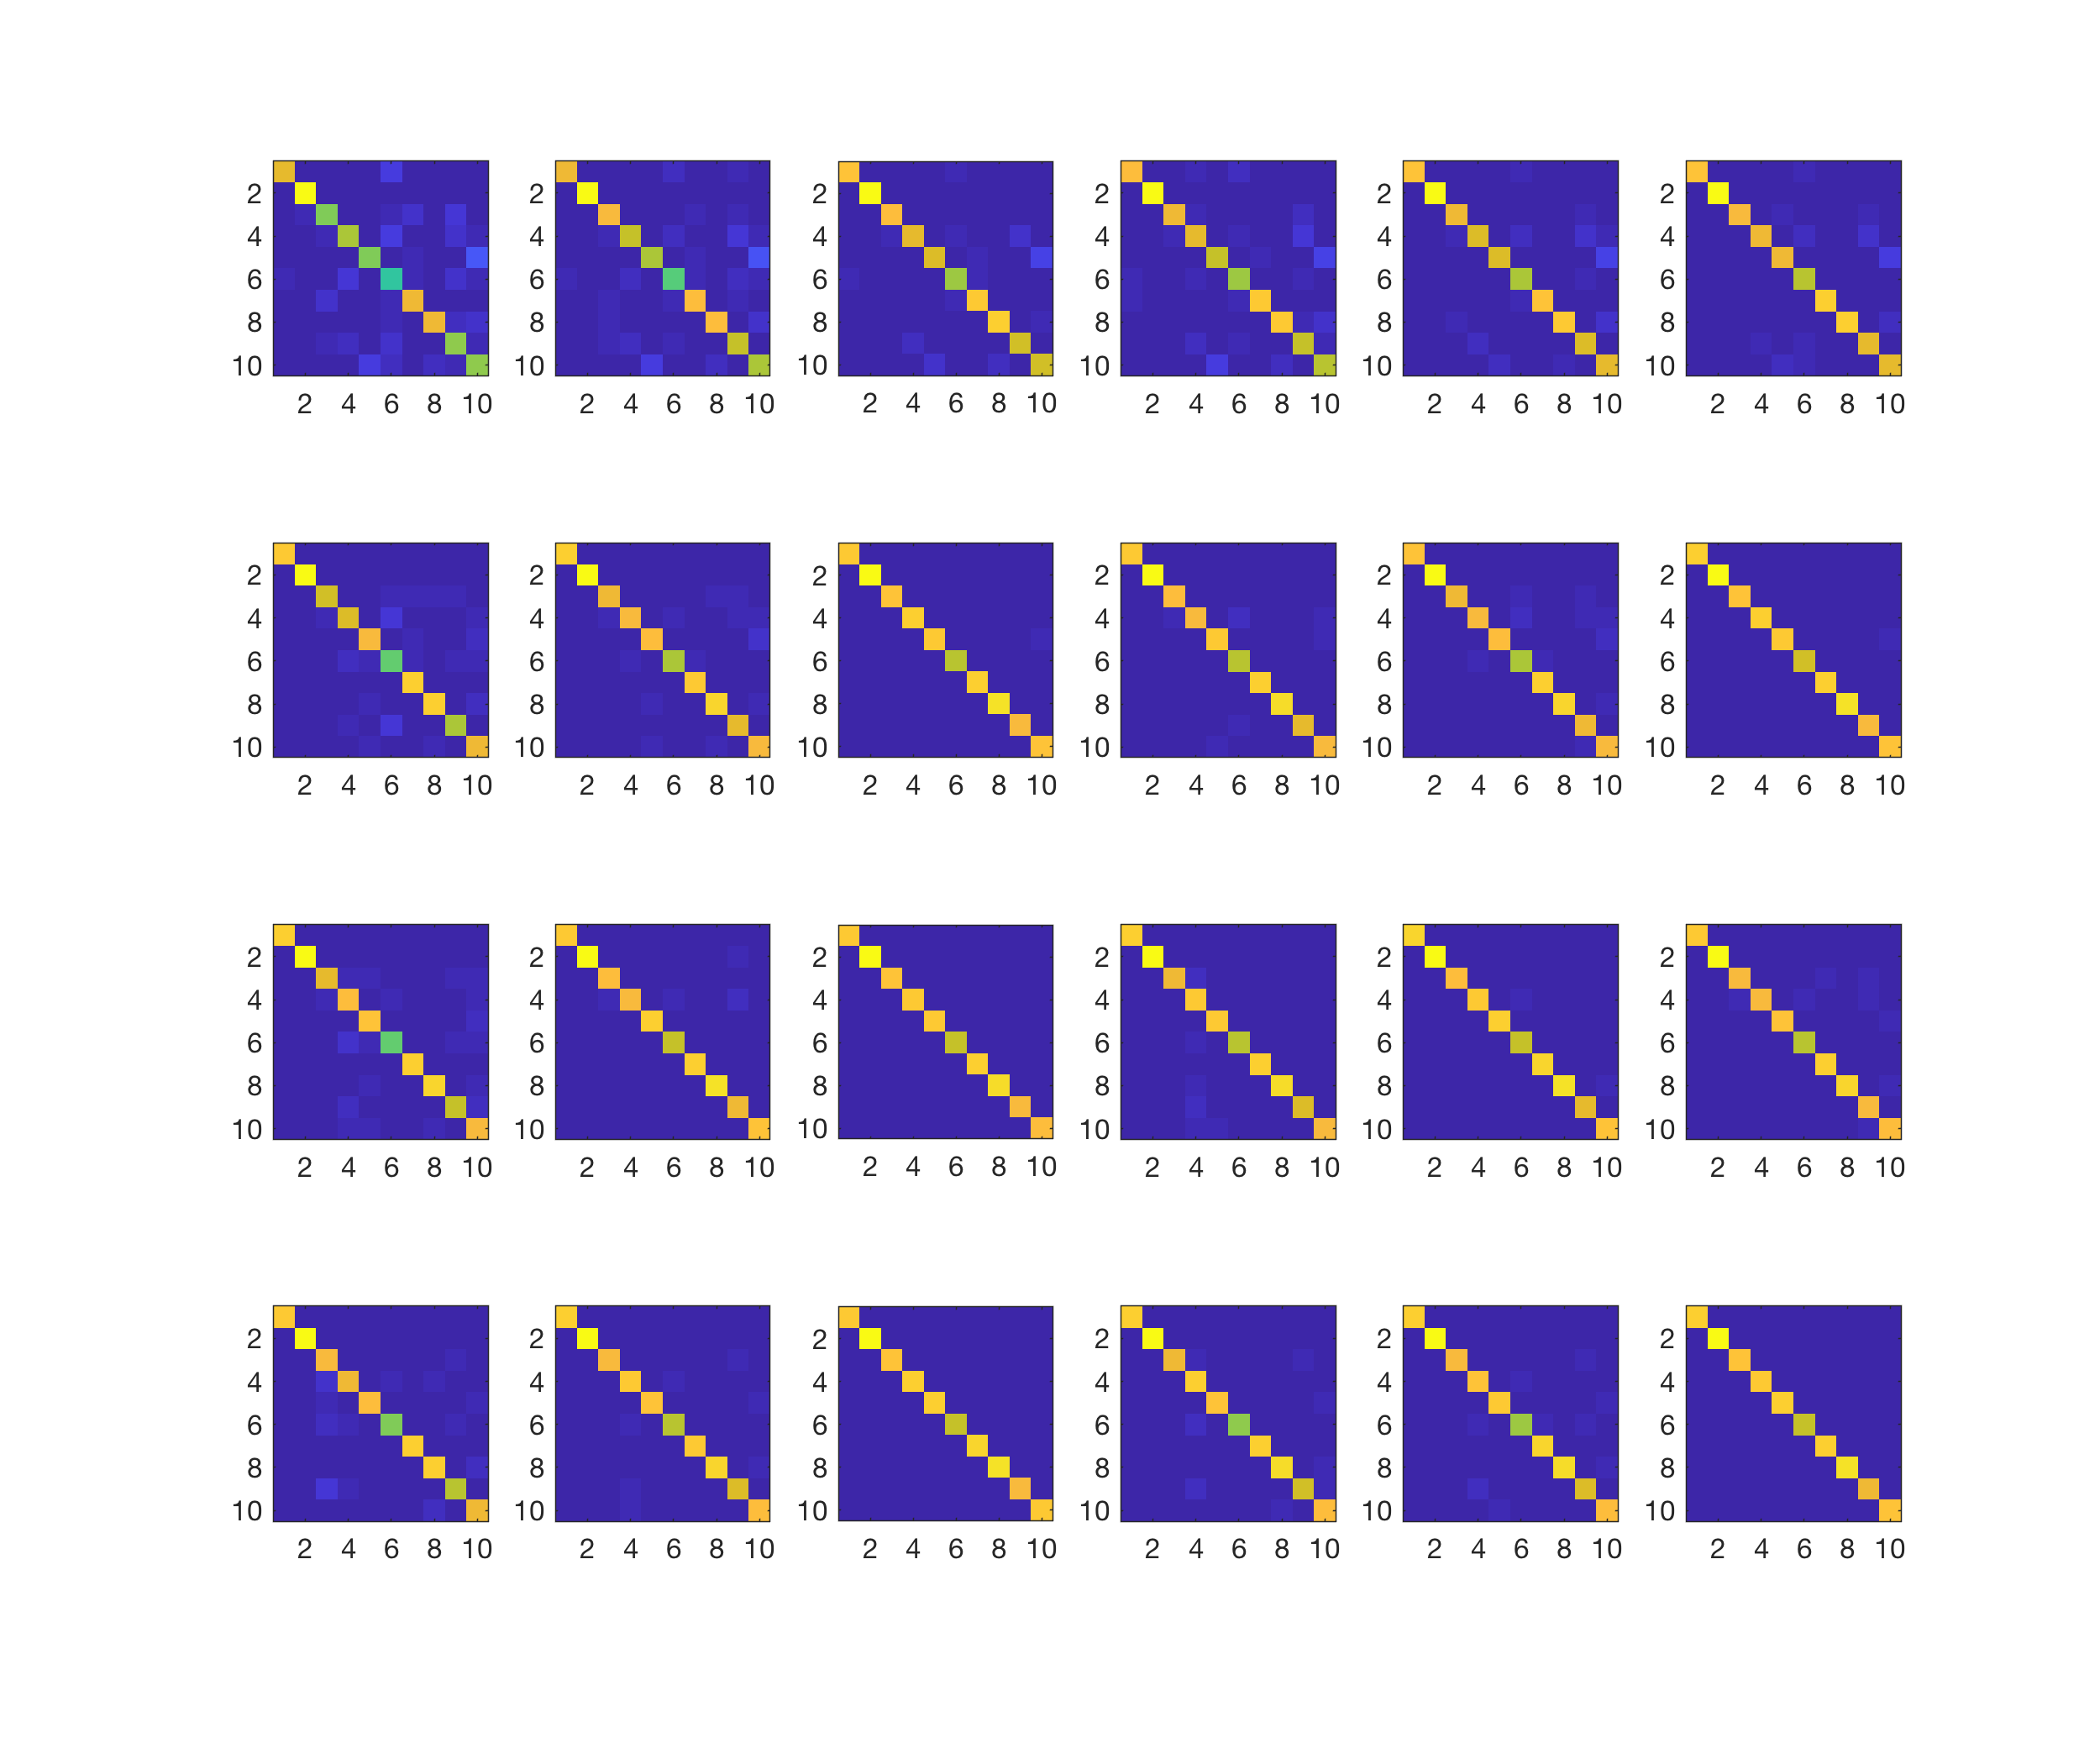
\includegraphics[width=0.9\linewidth]{PCA_1DNN_MNIST}
\caption{Missclassification matrices. Each row represents an agreed level of explained variance in ascending order (50\%, 75\%, 85\%, 95\%) and each column represents a neural network architecture in the order of increasing complexity (10; 25; 100; 25 $\rightarrow$ 15; 25 $\rightarrow$ 20 $\rightarrow$ 15; 100 $\rightarrow$ 50 $\rightarrow$ 20)}
\label{fig:PCA_1DNN_MNIST}
\end{figure}

\begin{table}[p]
\centering
  \begin{tabular}{|cc|l|c|c|}
  	\hline
    \% Var & PCs & NN Architecture & Training Error & Test Error \\
    \hline
    \hline
    50 & 11 & 25 & 0.168   &  0.698 \\
    50 & 11 & 25-20-15 & 0.119  &   0.838  \\
    \hline
    75 & 33 & 25 & 0.088  &   0.729 \\
    75 & 33 & 100 &    0.037  &   0.817\\
    \hline
    85 & 58 & 10 & 0.084  &   0.705\\
    85 & 58 & 25-20-15 & 0.066  &   0.807\\
    \hline
    95 & 150 & 25 &  0.054   &  0.688\\
    95 & 150 & 100-50-20 & 0.049   &  0.852\\
    \hline
  \end{tabular}
  \vspace{0.5em}
  \caption{Best and worst results for different PCA sizes depending on explanatory power of the variance. Training size: 9000 images. Test size: 1000 images.}
\end{table}

\begin{figure}[p]
\centering
\textbf{Results: PCA + FCNN on notMNIST dataset}
  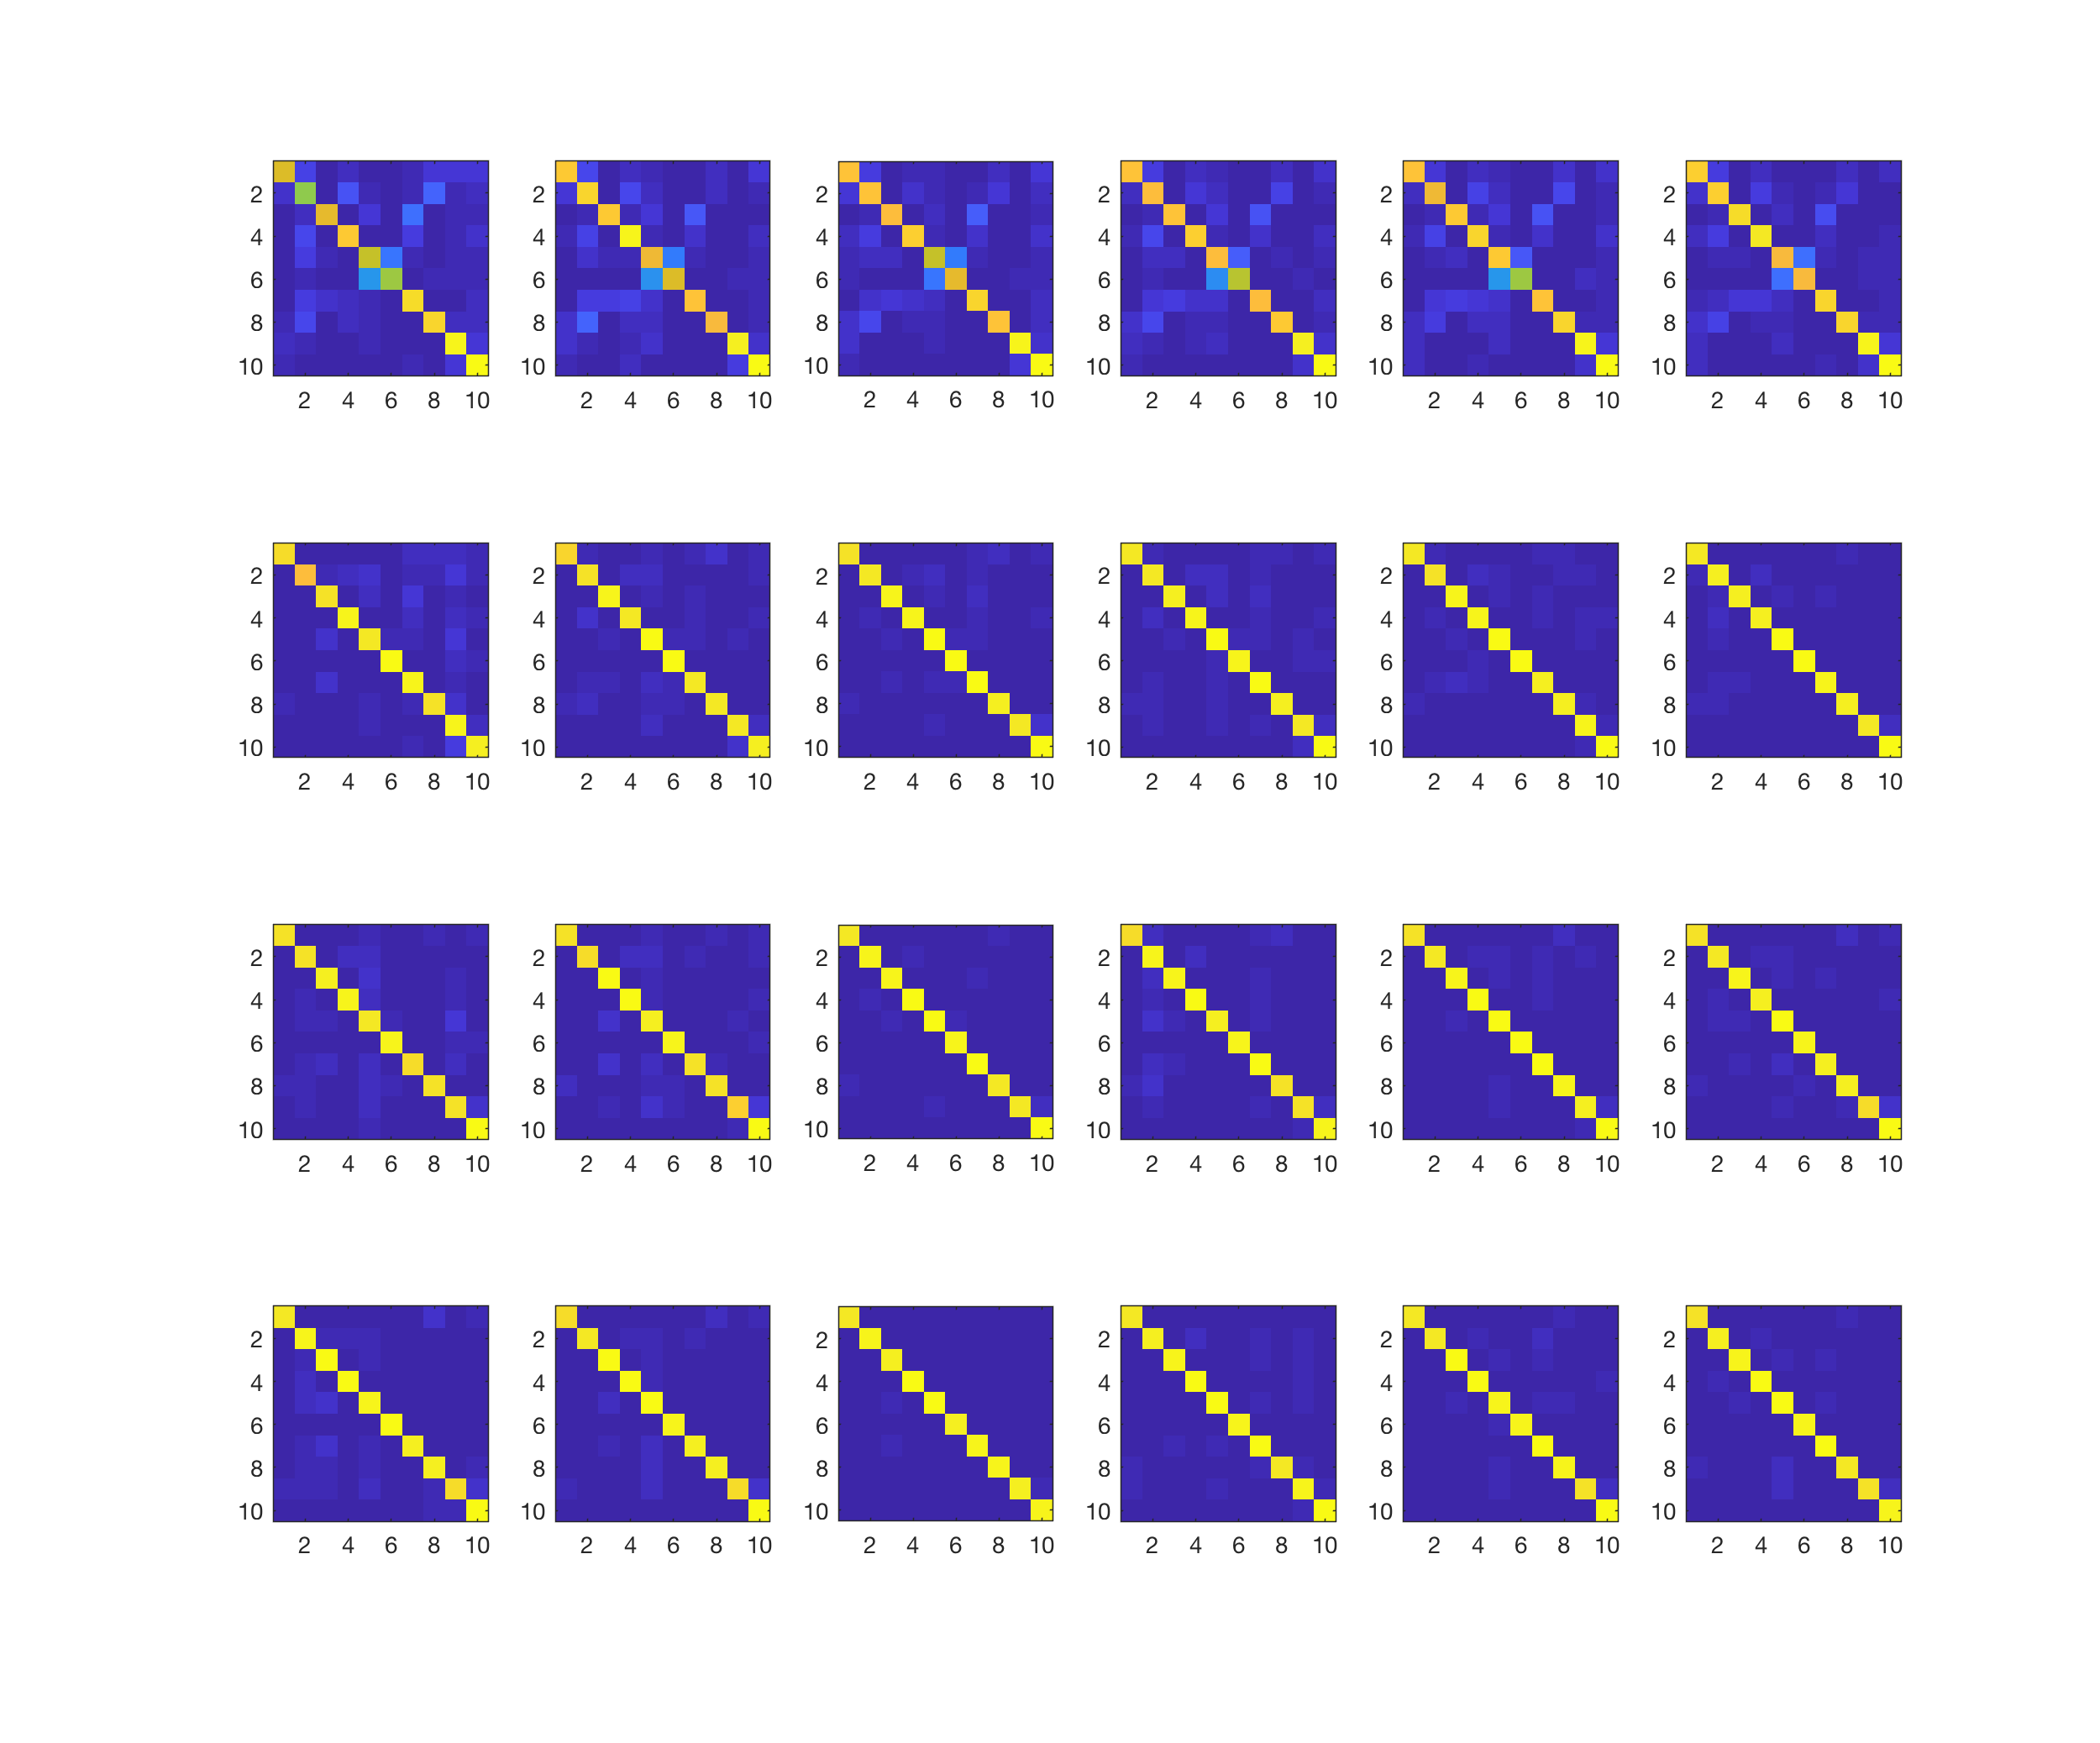
\includegraphics[width=0.9\linewidth]{PCA_1DNN_notMNIST}
\caption{Missclassification matrices. Each row represents an agreed level of explained variance in ascending order (50\%, 75\%, 85\%, 95\%) and each column represents a neural network architecture in the order of increasing complexity (10; 25; 100; 25 $\rightarrow$ 15; 25 $\rightarrow$ 20 $\rightarrow$ 15; 100 $\rightarrow$ 50 $\rightarrow$ 20)}
\label{fig:PCA_1DNN_notMNIST}
\end{figure}

\begin{table}[p]
\centering
  \begin{tabular}{|cc|l|c|c|}
  	\hline
    \% Var & PCs & NN Architecture & Training Error & Test Error \\
    \hline
    \hline
    50 & 5 & 100-50-20 & 0.207    & 0.612\\
    50& 5 & 25-20-15 & 0.235    & 0.639\\
    \hline
    75 & 19 &  100 & 0.089    & 0.555\\
    75 & 19& 25-20-15 & 0.104    & 0.642\\
    \hline
    85 & 40 & 25 & 0.101   &  0.559\\
    85 & 40 & 100-50-20 & 0.094     & 0.62\\
    \hline
    95 & 126 & 25-20-15 & 0.089   &  0.568\\
    95 & 126 & 25-15 & 0.081   &  0.587\\
    \hline
  \end{tabular}
    \vspace{0.5em}
  \caption{Best and worst results for different PCA sizes depending on explanatory power of the variance. Training size: 9000 images. Test size: 1000 images.}
\end{table}

\begin{figure}[p]
\centering
\textbf{Results: PCA + FCNN on Fashion MNIST dataset}
  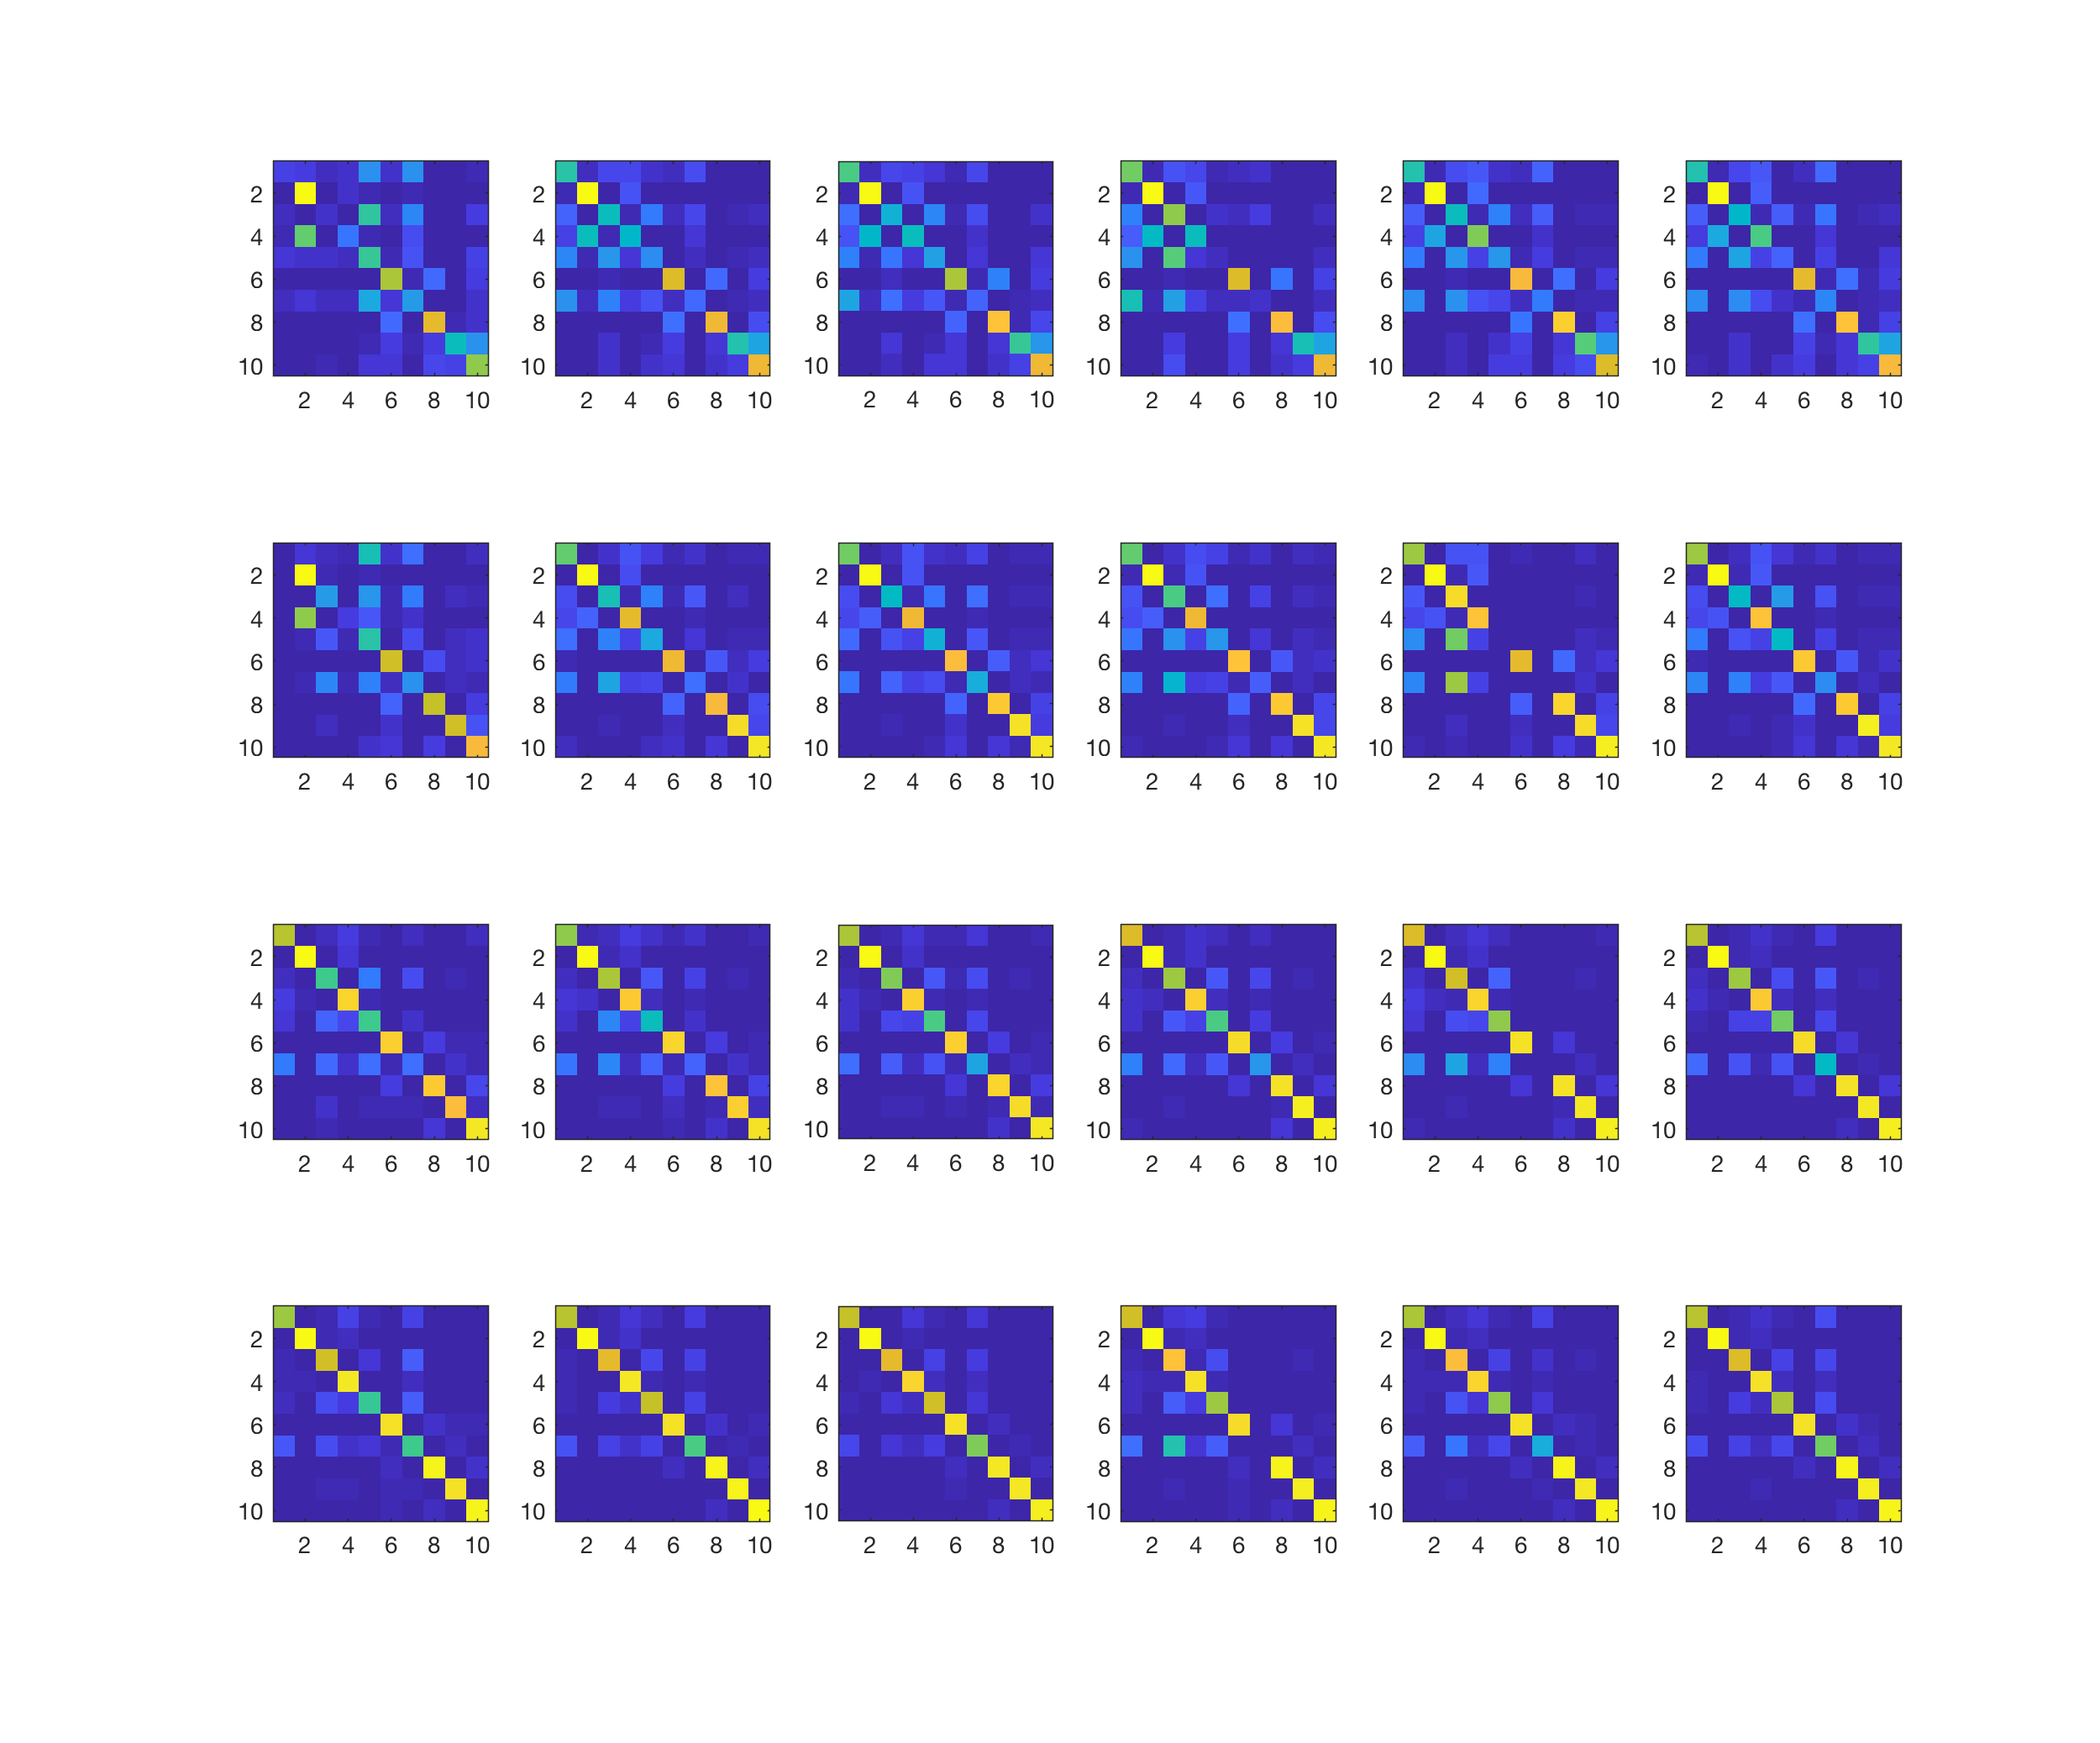
\includegraphics[width=0.9\linewidth]{PCA_1DNN_Fashion_MNIST}
\caption{Missclassification matrices. Each row represents an agreed level of explained variance in ascending order (50\%, 75\%, 85\%, 95\%) and each column represents a neural network architecture in the order of increasing complexity (10; 25; 100; 25 $\rightarrow$ 15; 25 $\rightarrow$ 20 $\rightarrow$ 15; 100 $\rightarrow$ 50 $\rightarrow$ 20)}
\label{fig:PCA_1DNN_Fashion_MNIST}
\end{figure}

\begin{table}[p]
\centering
  \begin{tabular}{|cc|l|c|c|}
  	\hline
    \% Var & PCs & NN Architecture & Training Error & Test Error \\
    \hline
    \hline
    50 &2 & 25-15 & 0.498     & 0.516\\
    50 & 2 & 10 & 0.52256     & 0.554\\
    \hline
    75 & 3 & 100 & 0.35622    &  0.398\\
    75 & 3 & 25 & 0.40367   &   0.422\\
    \hline
    85 & 8 & 100-50-20 & 0.22089    &  0.257\\
    85 & 8 & 10 & 0.28756    &  0.327\\
    \hline
    95 & 44 & 25-15 & 0.17978    &  0.399 \\
    95 & 44 & 100 & 0.151   &   0.444\\
    \hline
  \end{tabular}
    \vspace{0.5em}
  \caption{Best and worst results for different PCA sizes depending on explanatory power of the variance. The dataset is preprocessed by doing 2D Fourier transform of each image. Training size: 9000 images. Test size: 1000 images.}
\end{table}

\subsection*{CNN}

Convolutional neural networks perform very well in our classification task. As expected the training and the test error decrease with increasing depth of the network. The results received are the opposite compared to PCA. The lowest test and training errors are received for the MNIST dataset and the highest for the Fashion MNIST dataset, as expected. However the size of the errors is much smaller than for the PCA approach. For instance, the deepest architecture yields a training error of smaller than 1\% for the MNIST dataset with a corresponding test error of approximately 3\%. Even with Fashion MNIST the highest test error received with the simplest network is still smaller than 18\%.

\begin{figure}[p]
\centering
\textbf{Results: CNN on all datasets\\}
\vspace{1em}
\begin{subfigure}{.3\textwidth}
  \centering
  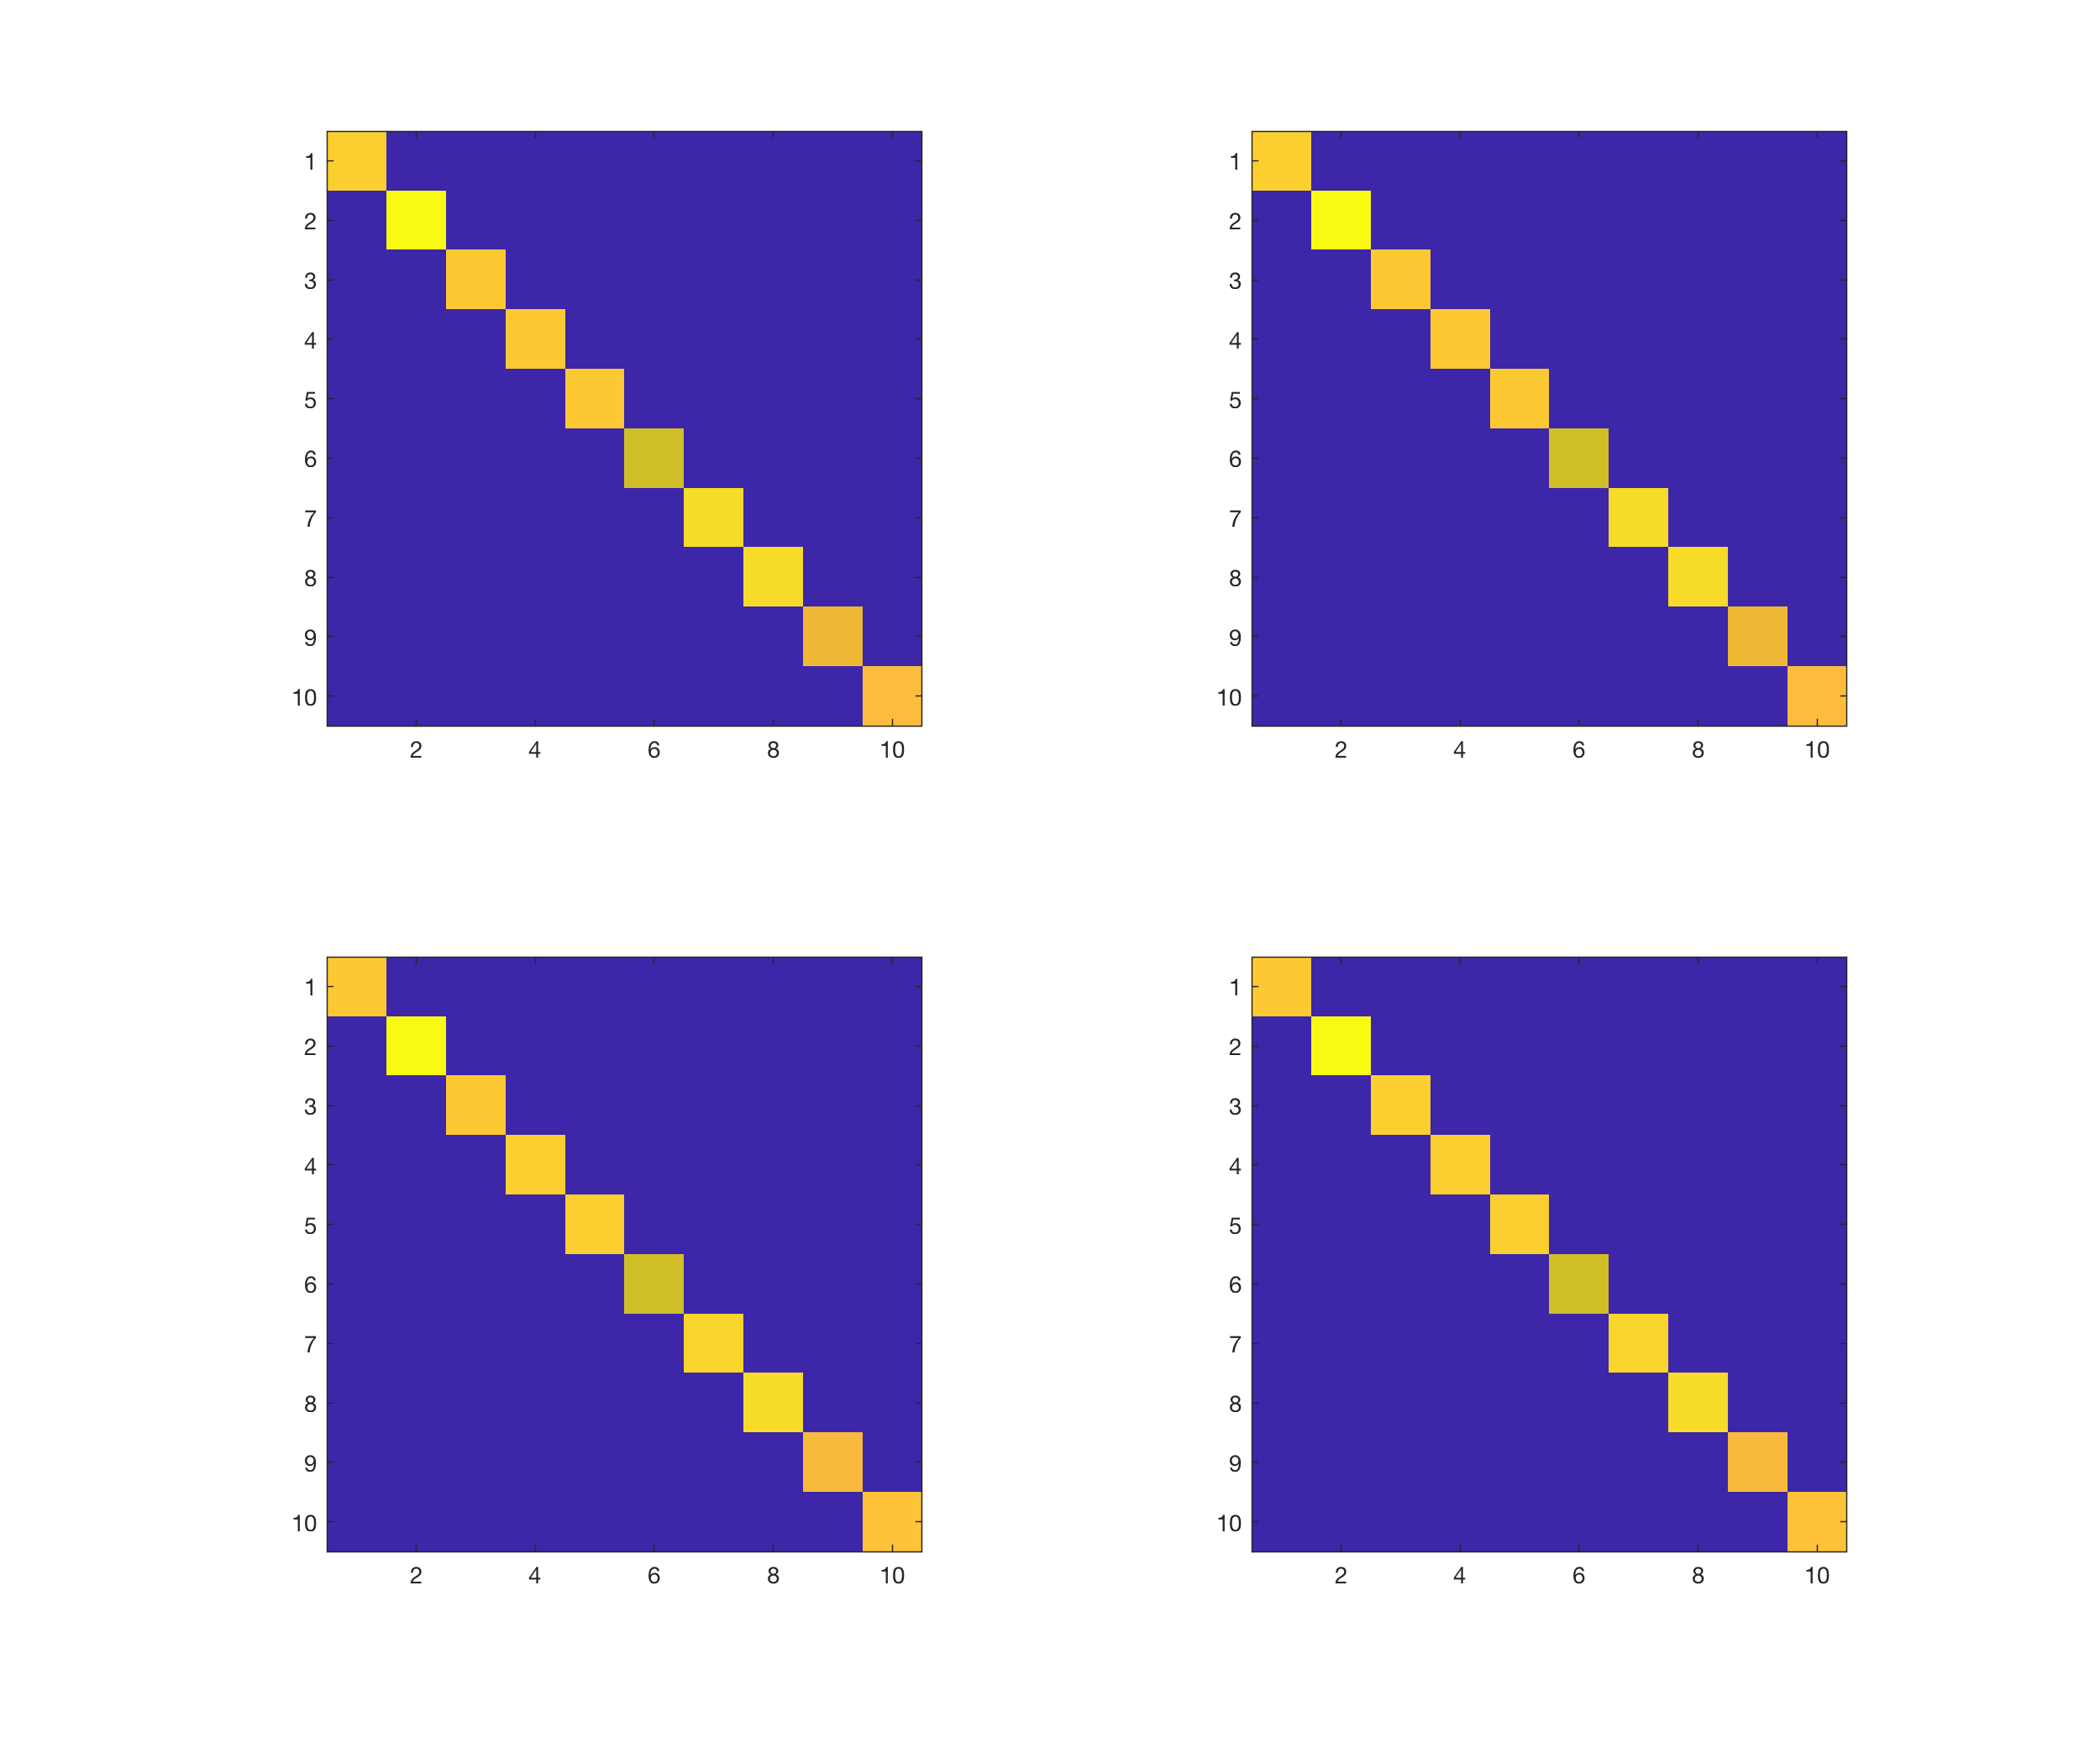
\includegraphics[width=\linewidth]{CNN_MNIST}
  \caption{~}
\end{subfigure}%
\begin{subfigure}{.3\textwidth}
  \centering
  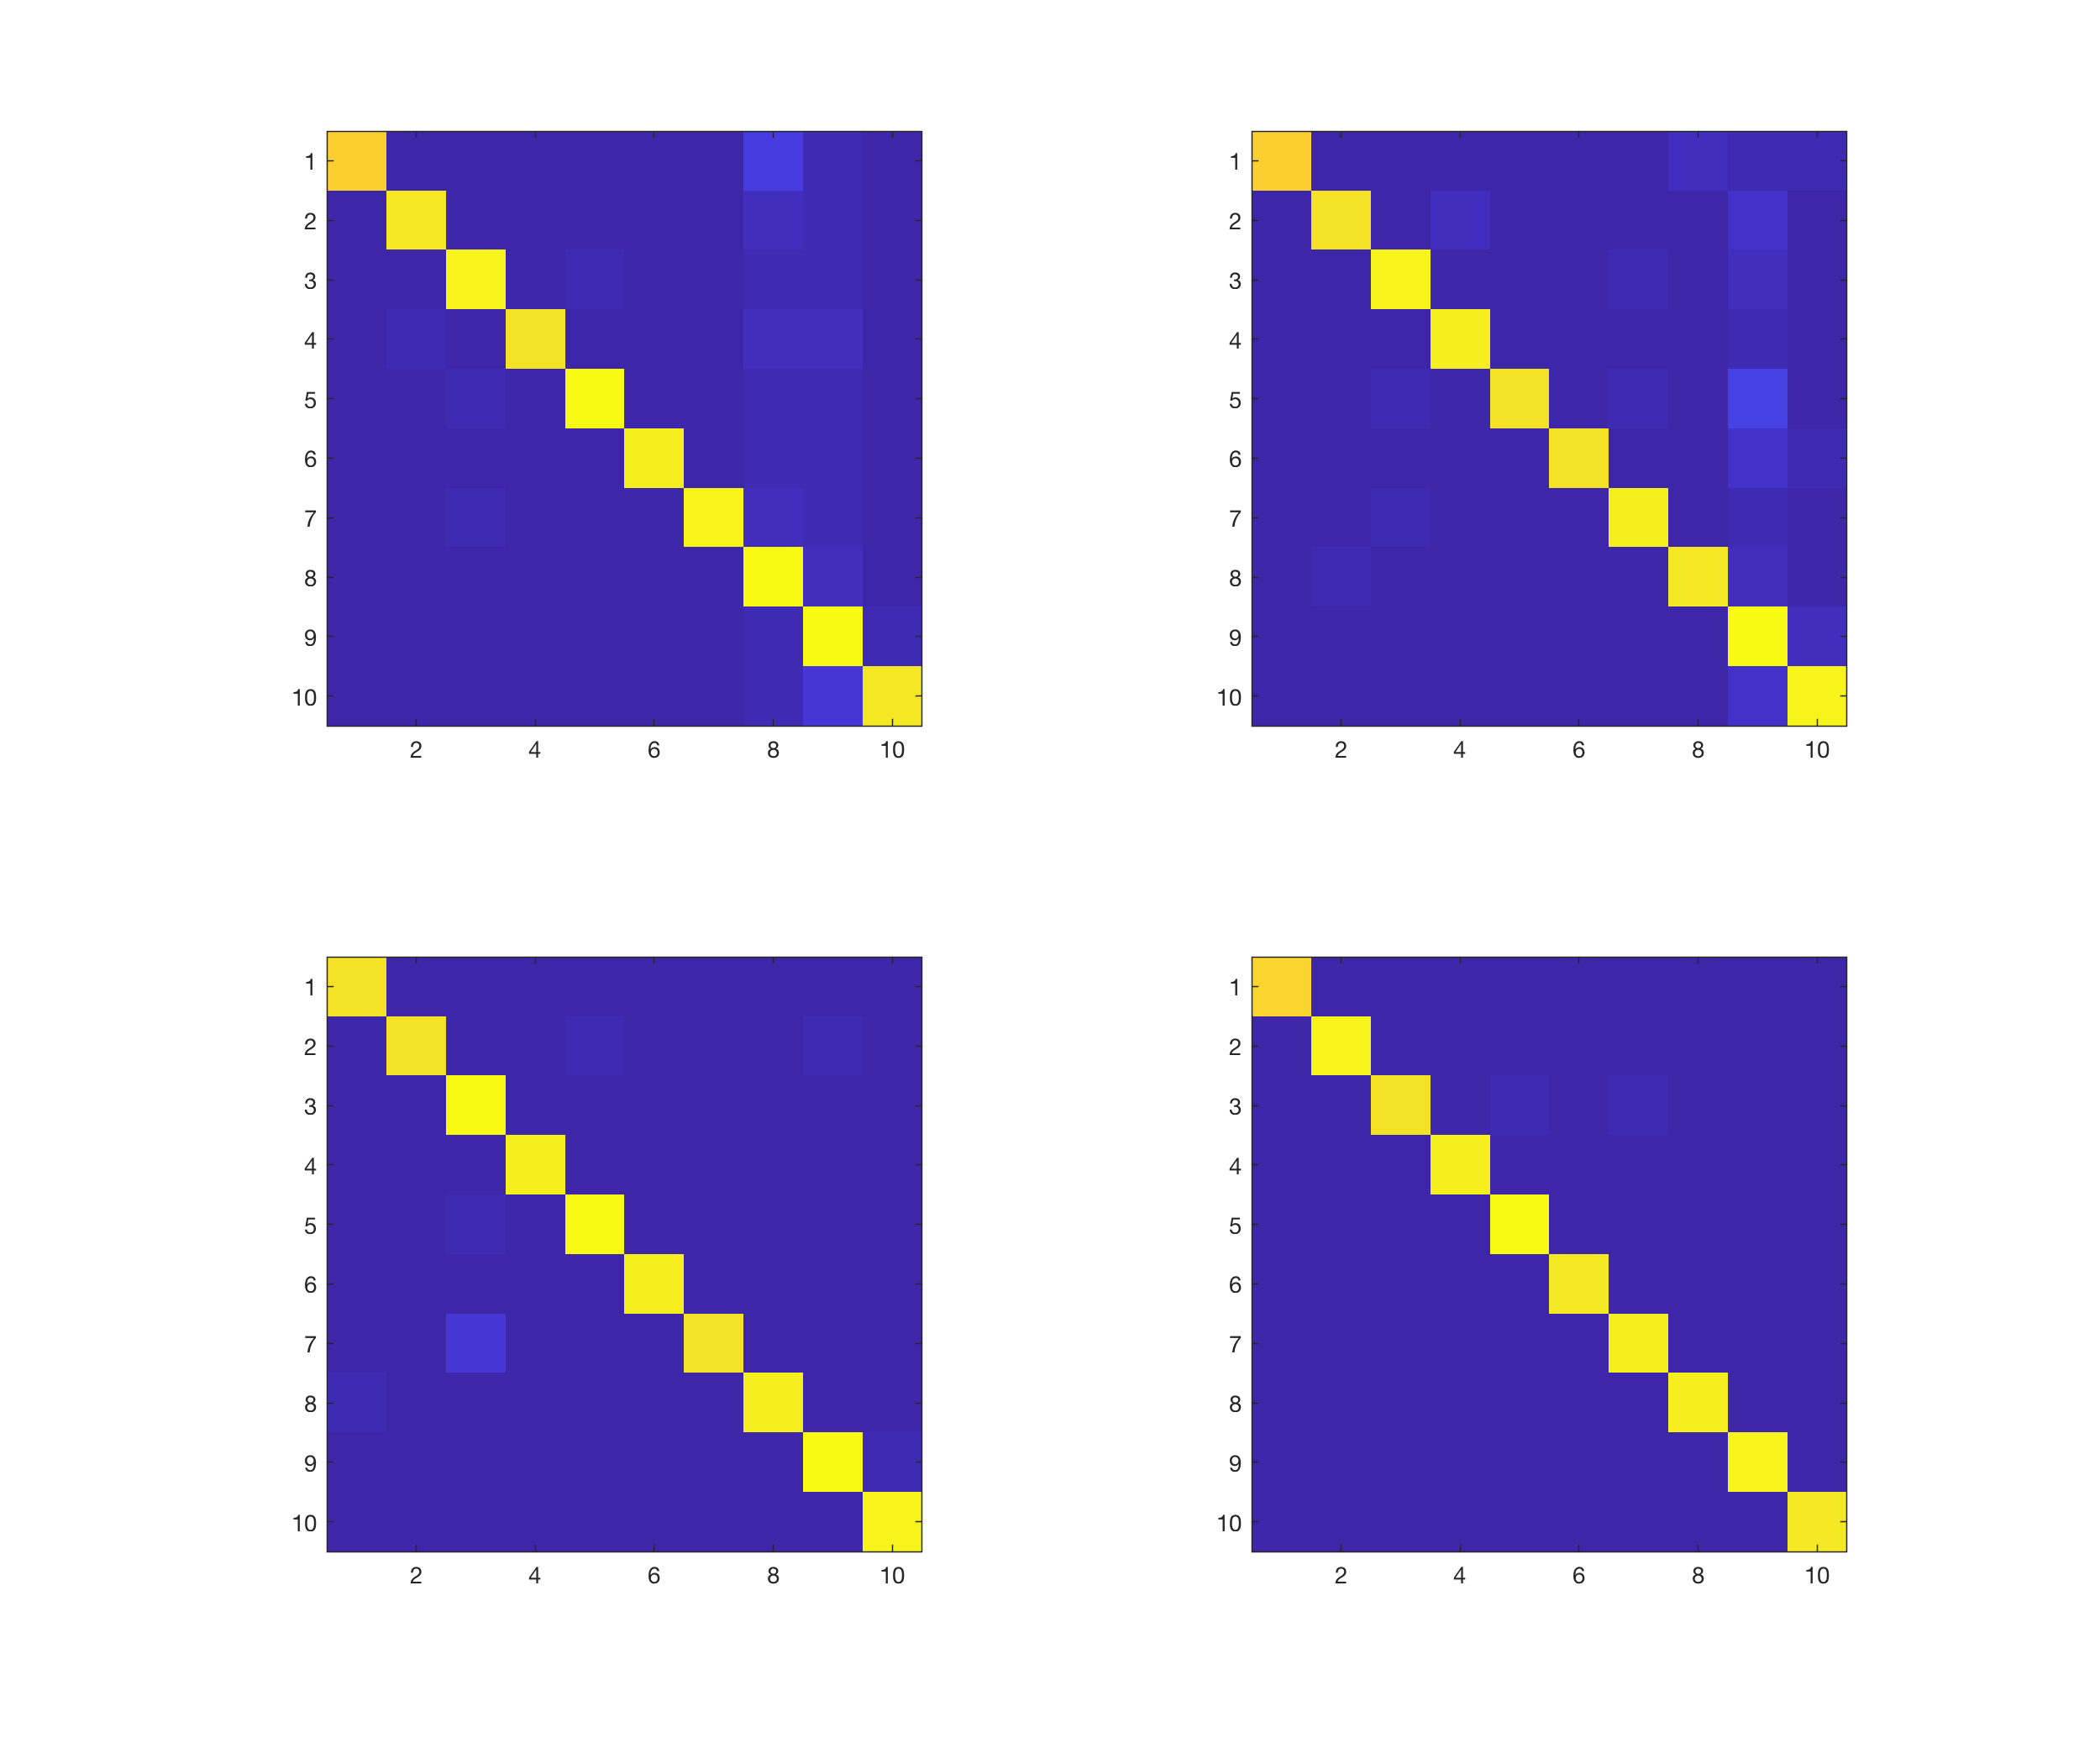
\includegraphics[width=\linewidth]{CNN_notMNIST}
  \caption{~}
\end{subfigure}
\begin{subfigure}{.3\textwidth}
  \centering
  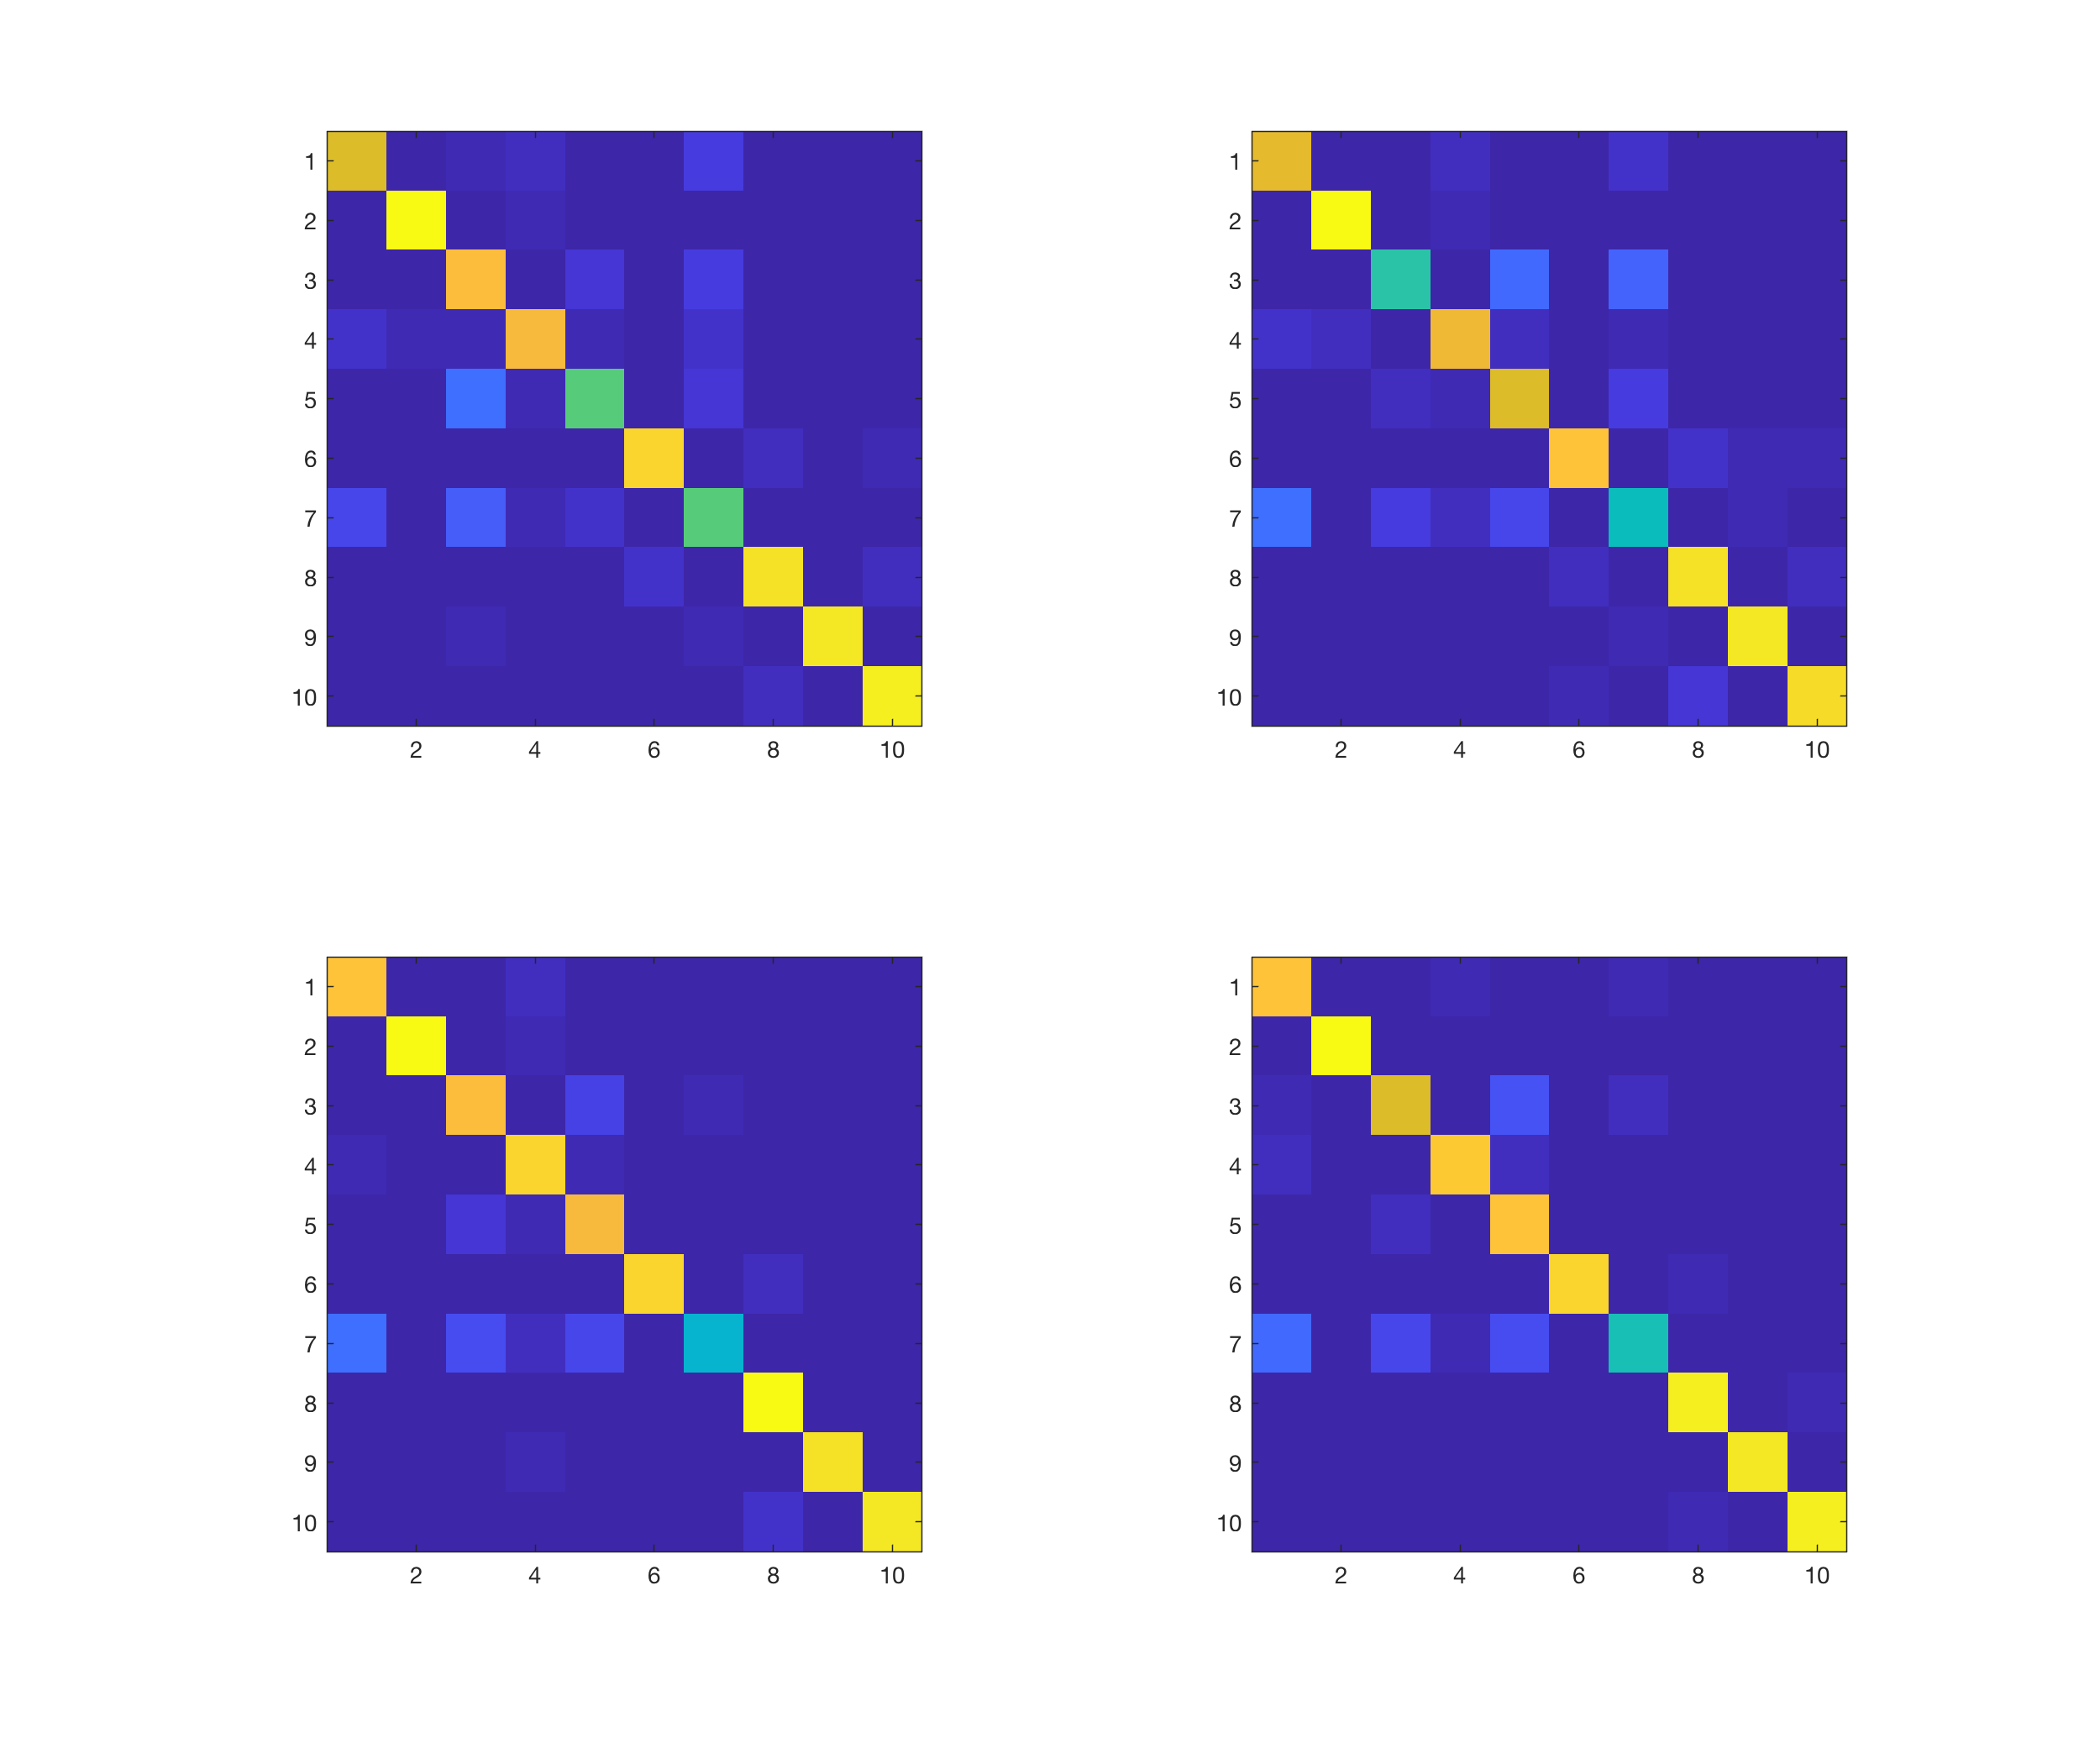
\includegraphics[width=\linewidth]{CNN_Fashion_MNIST}
  \caption{~}
\end{subfigure}
\caption{Missclassification matrices for the CNNs, with architectures in order [1,2; 3,4]. (a) MNIST; (b) notMNIST; (c) Fashion MNIST.}
\label{fig:jj}
\end{figure}

\begin{table}[p]
\centering
  \begin{tabular}{|c|l|c|c|}
  	\hline
    \# & CNN Architecture & Training Error & Test Error\\
    \hline
    \hline
        1 & 2D(5x5,4)  &                 0.025625   &  0.055\\     
    2 & 2D(5x5,8)  &               0.020375  &   0.049  \\   
    3 & 2D(3x3,4)-BN      &          0.002125  &   0.045   \\  
    4 & 2D(3x3,8)-BN-2D(5x5,16)-BN      &        0.001625  &   0.031 \\
    \hline
  \end{tabular}
  \vspace{0.5em}
  \caption{CNNs on MNIST. {Training size: 9000 images (10\% for validation). Training options: Stochastic Gradient Descent with Momentum, maximum 20 epochs with validation patience of 10 epochs, Mini Batch size of 64, L2 regularization factor of 0.0005.}}
\end{table}

\begin{table}[p]
\centering
  \begin{tabular}{|c|l|c|c|}
  	\hline
    \# & CNN Architecture & Training Error & Test Error\\
    \hline
    \hline
       1 & 2D(5x5,4)     &              0.08275   &  0.112  \\   
   2 & 2D(5x5,8)   &         0.08125     &0.108  \\   
    3 & 2D(3x3,4)-BN     &       0.044875    & 0.099 \\    
    4 & 2D(3x3,8)-BN-2D(5x5,16)-BN     &        0.0415    & 0.088   \\
    \hline
  \end{tabular}
  \vspace{0.5em}
  \caption{CNNs on notMNIST. {Training size: 9000 images (10\% for validation). Training options: Stochastic Gradient Descent with Momentum, maximum 20 epochs with validation patience of 10 epochs, Mini Batch size of 64, L2 regularization factor of 0.0005.}}
\end{table}

\begin{table}[p]
\centering
  \begin{tabular}{|c|l|c|c|}
  	\hline
    \# & CNN Architecture & Training Error & Test Error\\
    \hline
    \hline
    1 & 2D(5x5,4)   &             0.16287    &  0.179     \\
    2 & 2D(5x5,8)   &            0.16225     & 0.168     \\
   3 & 2D(3x3,4)-BN   &           0.1035      &0.148   \\  
    4 & 2D(3x3,8)-BN-2D(5x5,16)-BN    &           0.10475      &0.144  \\
    \hline
  \end{tabular}
  \vspace{0.5em}
  \caption{CNNs on Fahion MNIST. {Training size: 9000 images (10\% for validation). Training options: Stochastic Gradient Descent with Momentum, maximum 20 epochs with validation patience of 10 epochs, Mini Batch size of 64, L2 regularization factor of 0.0005.}}
\end{table}

\section{Conclusions}
We find that convolutional neural networks highly outperform principal component analysis for simple as well as for more complex datasets. Also, results achieved by means of FCNNs are, even for "deep" architectures, simply not comparable to those of CNNs, which even with 1 convolutional layer show very high classification accuracy. \\
As it is to be expected, MNIST proves the easiest task in the pool of our datasets of choice, while Fashion MNIST, with its non-trivial visual features, is the hardest one.

%++++++++++++++++++++++++++++++++++++++++
% References section will be created automatically 
% with inclusion of "thebibliography" environment
% as it shown below. See text starting with line
% \begin{thebibliography}{99}
% Note: with this approach it is YOUR responsibility to put them in order
% of appearance.

% \begin{thebibliography}{99}

% \bibitem{melissinos}
% A.~C. Melissinos and J. Napolitano, \textit{Experiments in Modern Physics},
% (Academic Press, New York, 2003).

% \bibitem{Cyr}
% N.\ Cyr, M.\ T$\hat{e}$tu, and M.\ Breton,
% % "All-optical microwave frequency standard: a proposal,"
% IEEE Trans.\ Instrum.\ Meas.\ \textbf{42}, 640 (1993).

% \bibitem{Wiki} \emph{Expected value},  available at
% \texttt{http://en.wikipedia.org/wiki/Expected\_value}.

% \end{thebibliography}


\end{document}
